\documentclass[14pt,a4paper,openany]{extbook}
\usepackage{times}

\usepackage[russian,english]{babel}

\usepackage{geometry}
\geometry{
    left=25mm,
    right=20mm,
    top=20mm,
    bottom=20mm
}

\usepackage{setspace}
\onehalfspacing

\setlength{\parindent}{1.25cm}
\setlength{\parskip}{0pt}

\usepackage{ragged2e}
\justifying

\usepackage{graphicx}
\usepackage{amsmath, amssymb}
\usepackage{booktabs}
\usepackage{longtable}

\usepackage{caption}

% Рисунки — подпись слева под рисунком
\captionsetup[figure]{
    justification=raggedright,
    singlelinecheck=false
}
\usepackage[font=small,labelfont=bf]{caption}

% Таблицы — подпись по центру НАД таблицей
\captionsetup[table]{
    justification=centering,
    singlelinecheck=false,
    position=top
}

% ---------- Сноски ----------
\renewcommand{\footnotesize}{\fontsize{12}{14}\selectfont}

% ---------- Библиография ----------
\usepackage[backend=biber,style=gost-numeric,sorting=none]{biblatex}
\addbibresource{references.bib}

% ---------- Оглавление ----------
\usepackage{tocloft}
\renewcommand{\cftchapfont}{\normalfont}
\renewcommand{\cftsecfont}{\normalfont}


% \title{Physics-Informed Neural Network Approach to Bacterial Growth Modeling}
% \author{Liubov Smirnova \\ Supervisor: Prof. Anna Maslovskaya}
% \date{}

\usepackage{pdfpages}
\begin{document}

\includepdf[pages=-]{title.pdf}

\chapter*{Abstract}
\addcontentsline{toc}{chapter}{Abstract}

This thesis develops and validates a Physics-Informed Neural Network (PINN)
framework for modelling bacterial growth and quorum sensing dynamics
governed by nonlinear ordinary differential equations. Built on
DeepXDE/PyTorch, the framework incorporates hard-constraint enforcement of
initial conditions, singularity-avoiding loss reformulations for Monod and
Hill kinetics, multiplicative variable scaling ($s=10^{7}$), anchor-point
data assimilation, and multi-stage Adam/L-BFGS optimisation.

Three experiments of increasing complexity validate the approach.
Experiment~1 (Monod chemostat) achieves sub-percent $L_2$ error against a
Radau~IIA reference in under 5~minutes on an NVIDIA Tesla~T4 GPU.
Experiment~2 (three-variable \textit{Pseudomonas putida} IsoF quorum
sensing network) captures all dynamical phases with $R^2>0.9999$ in
8.5~minutes. Experiment~3 recovers two hidden parameters from 40~noisy
observations (3\% Gaussian noise) with sub-1\% relative error in
26~minutes, without external optimisation wrappers.

The results demonstrate that domain-adapted PINNs provide a unified tool
for forward simulation, data assimilation, and parameter inference in
microbial systems, with a modular methodology transferable to other
ODE-governed biological processes.

\bigskip
\noindent\textbf{Keywords:} physics-informed neural networks, bacterial
growth modelling, quorum sensing, inverse problems, parameter estimation,
ordinary differential equations, DeepXDE, \textit{Pseudomonas putida}

\newpage
\tableofcontents
\newpage
\listoffigures

\chapter{Introduction}
\label{chap:intro}
\chaptermark{Introduction}

Understanding and predicting bacterial growth dynamics represents a cornerstone of microbiology with far-reaching implications across biomedical, environmental, and industrial domains. Bacterial populations do not merely grow in isolation; they engage in complex social behaviours, communicate via small diffusible signalling molecules in a process known as quorum sensing~\cite{mukherjee2019bacterial}, and frequently form structured, surface-associated communities termed biofilms. These biofilms are notorious for their heightened tolerance to antimicrobial agents, contributing significantly to the global crisis of antibiotic resistance. The World Health Organization has identified antimicrobial resistance---intrinsically linked to biofilm-mediated persistence---as one of the top ten global public health threats, underscoring the urgent need for advanced predictive models that can inform intervention strategies and guide the rational design of antimicrobial therapies.

The mathematical modelling of microbial population dynamics has evolved over more than a century, progressing from simple empirical growth curves to sophisticated mechanistic frameworks that capture nutrient limitation, physiological adaptation, and cell-to-cell communication. The trajectory began with phenomenological descriptions such as the logistic equation, which represents self-limiting growth through a single carrying-capacity parameter. A major conceptual advance was the Monod equation, which mechanistically linked the specific growth rate to the extracellular concentration of a limiting substrate via saturation kinetics analogous to the Michaelis--Menten model in enzymology. The Monod framework, when embedded in a continuous-culture (chemostat) mass balance, forms the basis for much of modern bioprocess engineering and remains the standard benchmark for validating new computational approaches---a role it plays in the present thesis as well (Chapter~\ref{chap:implementation}, Experiment~1). Further refinement came with models such as that of Baranyi and Roberts~\cite{baranyi1994}, which introduced a physiological-state adjustment function to dynamically capture the lag phase---the period of metabolic adaptation that bacteria undergo when transferred to a new environment---providing a more accurate description of the full growth curve from inoculation to stationary phase.

Despite these advances, classical models often struggle with three interrelated challenges that arise in real-world biological systems. First, the inherent multi-scale nature of microbial processes---where molecular signalling events on the nanomolar scale coexist with population-level dynamics on the milligram-per-millilitre scale---creates severe numerical stiffness that taxes conventional solvers. Second, model parameters (growth rates, decay constants, Hill coefficients) are rarely known \textit{a priori} and must be estimated from experimental measurements that are typically sparse, irregularly sampled, and corrupted by noise. Third, the emergence of complex collective behaviours, such as the coordinated gene expression in quorum sensing that regulates virulence factor production and biofilm formation in pathogens like \textit{Pseudomonas aeruginosa}~\cite{buddrus2014analysis}, demands modelling approaches that can seamlessly integrate intracellular regulatory networks with population-level mass balances and heterogeneous experimental data.

A particularly acute methodological gap lies in the solution of inverse problems, where the goal is to infer unknown model parameters from observed trajectories. Conventional numerical methods for ordinary differential equations (ODEs)---whether explicit Runge--Kutta schemes or implicit methods such as Radau~IIA---are designed for forward simulation: given parameters and initial conditions, they produce trajectories. Parameter estimation requires wrapping these solvers inside external optimisation algorithms (e.g., Nelder--Mead, genetic algorithms, Markov chain Monte Carlo), each forward evaluation demanding a complete numerical integration of the ODE system. For complex models with many unknowns, this nested optimisation becomes computationally prohibitive and algorithmically cumbersome, creating a practical barrier between mechanistic theory and experimental observation.

In recent years, a promising approach has emerged at the intersection of machine learning and scientific computing: Physics-Informed Neural Networks (PINNs), introduced by Raissi, Perdikaris, and Karniadakis~\cite{raissi2019}. PINNs embed the governing physical laws---expressed as differential equations---directly into the loss function of a neural network, so that the optimiser simultaneously minimises the ODE (or PDE) residual across the computational domain and fits any available experimental data. This formulation offers two structural advantages over classical solvers. For forward problems, PINNs operate in a mesh-free manner: the network learns a continuous, differentiable representation of the solution without constructing a time grid, thereby avoiding the sequential error accumulation and step-size limitations inherent in time-stepping methods. For inverse problems, unknown parameters are simply declared as additional trainable variables and optimised alongside the network weights in a single training pass, eliminating the need for external optimisation wrappers. PINNs have been applied successfully to fluid mechanics, heat transfer, and solid mechanics, but their systematic application to microbial growth and signalling models---with their characteristic stiffness, extreme scale disparity, and fractional-order nonlinearities---remains largely unexplored.

The primary objective of this thesis is to bridge this methodological gap by developing, implementing, and rigorously validating a PINN-based computational framework for modelling bacterial growth and quorum sensing dynamics. The framework is built on the DeepXDE library~\cite{lu2021deepxde} with a PyTorch backend and is designed to handle both forward simulation and inverse parameter estimation within a unified code structure. The target biological systems span a deliberately chosen complexity gradient: the Monod chemostat, a smooth two-variable benchmark with an analytical steady state, and the \textit{Pseudomonas putida} IsoF quorum sensing model, a stiff three-variable system with eight orders of magnitude of scale disparity, a fractional Hill exponent, and delayed negative feedback through enzymatic signal degradation.

To achieve the stated objective, the following systematic research tasks have been formulated:

\begin{enumerate}
    \item Conduct a systematic review and critical analysis of existing mathematical frameworks for modelling bacterial growth dynamics, encompassing classical population models (logistic, Monod, Contois), mechanistic frameworks incorporating physiological states (Baranyi--Roberts), and modern approaches for collective behaviours (quorum sensing ODE models). The review identifies the limitations of each framework and the specific integration points where neural network methodologies can add value.

    \item Investigate and rigorously evaluate the PINN paradigm as a methodology for solving systems of ODEs relevant to microbiology, with particular emphasis on the techniques required to handle biological specifics: hard-constraint enforcement of initial conditions, singularity-avoiding loss reformulations for saturation kinetics, variable normalisation for multi-scale systems, and multi-stage optimisation protocols combining first-order (Adam) and quasi-Newton (L-BFGS) methods.

    \item Design, implement, and validate a PINN-based software tool capable of simulating ODE systems describing both population growth and quorum sensing dynamics, and of inferring unknown biological parameters from sparse, noisy observations. Performance is assessed through \textit{in silico} experiments that quantify numerical accuracy (via $L_2$ relative error against high-precision Radau~IIA reference solutions), parameter identifiability (via recovery of known ground-truth values from synthetic data), and computational efficiency (via wall-clock training and inference times on consumer-grade GPU hardware).
\end{enumerate}

The methodological approach centres on the implementation of PINNs using Python within the DeepXDE/PyTorch ecosystem. Reference solutions for benchmarking are generated using the implicit Runge--Kutta method of the Radau~IIA family (fifth order, L-stable), computed in double precision with stringent tolerances ($\texttt{rtol} = 10^{-8}$, $\texttt{atol} = 10^{-11}$) to ensure that the numerical reference itself introduces negligible error. PINN training employs fully connected neural networks with $\tanh$ activation, Glorot normal initialisation, and a two-to-four-stage optimisation protocol that combines Adam with learning rate annealing and L-BFGS refinement. This comparative framework enables systematic verification of PINN accuracy against established numerical techniques, while facilitating quantitative assessment of convergence behaviour, error dynamics, and computational cost across problems of varying scale and complexity.

The scientific relevance of this research is substantiated by the critical importance of understanding and predicting bacterial growth mechanisms in contexts that span multiple disciplines. In biomedicine, biofilm-associated infections account for an estimated 65--80\% of all microbial infections in humans, contributing to persistent conditions involving medical implants, chronic wounds, and dental pathologies; the development of predictive models for biofilm formation and quorum sensing dynamics is therefore directly relevant to the design of anti-biofilm therapies and the management of chronic infections. In engineering, biofilm-induced material degradation represents a substantial economic burden, with marine infrastructure corrosion alone costing an estimated \$80--120 billion annually worldwide, while biofouling in industrial water systems, heat exchangers, and processing facilities leads to significant energy losses and maintenance expenditures. In environmental science, microbial contamination in water distribution systems and the role of biofilms in biogeochemical cycling pose ongoing challenges for public health protection and ecosystem management. In food technology, bacterial contamination on processing surfaces contributes to product spoilage and safety concerns, while simultaneously presenting opportunities for beneficial applications in bioremediation and industrial bioprocessing. Across all of these domains, the ability to simulate microbial dynamics accurately, to estimate hidden biological parameters from limited measurements, and to do so with computational efficiency on accessible hardware addresses a concrete and widely recognised need.

The PINN-based framework developed in this thesis addresses critical limitations of current modelling approaches along four axes. It provides enhanced predictive capability by accurately simulating complex bacterial behaviours---including stiff multi-scale dynamics, nonlinear feedback, and delayed enzymatic responses---under the physically consistent constraints imposed by the governing differential equations. It enables efficient parameter estimation by solving inverse problems in a single training pass, without the nested optimisation loops required by conventional methods. It achieves practical computational efficiency by completing all training runs in under 30 minutes on a consumer-grade Tesla T4 GPU, making the approach accessible to research groups without high-performance computing infrastructure. And it contributes a methodological advance by demonstrating, for the first time in a systematic and reproducible manner, that PINNs equipped with biologically informed architectural choices can handle the specific numerical challenges---scale disparity, fractional kinetics, stiffness---that have historically limited the application of neural network methods to mechanistic microbiology.

This thesis is organised into four main chapters followed by concluding remarks. Chapter~\ref{chap:litreview} presents a systematic review of bacterial growth modelling, from classical Monod kinetics through quorum sensing regulatory networks, and surveys the PINN literature with emphasis on biological applications, identifying the specific methodological gaps that motivate the present work. Chapter~\ref{chap:methodology} develops the complete mathematical and computational framework: governing equations for both target systems, the PINN architecture and loss function design, hard-constraint initial-condition enforcement, singularity-avoiding loss reformulations, variable normalisation for multi-scale problems, and the multi-stage optimisation protocol. Chapter~\ref{chap:implementation} reports the full experimental validation cycle, comprising three experiments of increasing complexity---forward Monod simulation, forward quorum sensing simulation, and inverse quorum sensing parameter estimation---with detailed quantitative comparison against Radau~IIA reference solutions. Chapter~\ref{chap:discussion} discusses the advantages, limitations, and future directions of the approach in the broader context of computational microbiology. The thesis concludes in Chapter~\ref{chap:conclusion} with a synthesis of key findings and an assessment of the framework's readiness for deployment on real experimental data.

The integration of mechanistic biological models with physics-informed machine learning, as developed and validated in this thesis, establishes a foundation for a new generation of computational tools in microbial systems biology. By demonstrating that a single framework can solve forward problems, assimilate sparse data, and infer hidden parameters---all while respecting the governing biophysics---this work contributes to the ongoing convergence of data-driven and model-driven approaches that is reshaping quantitative biology.

\chapter{Literature Review}
\label{chap:litreview}
\chaptermark{Literature Review}

This chapter surveys the theoretical and experimental foundations upon which the present thesis builds. The review is organised along a trajectory of increasing biological and mathematical complexity: from classical single-species growth models (Section~\ref{sec:growthmodels}), through the social behaviours that emerge when bacteria communicate via quorum sensing (Section~\ref{sec:quorum}), to the spatial organisation of biofilms and its implications for antibiotic resistance (Section~\ref{sec:biofilms}). Section~\ref{sec:experiments} examines the experimental techniques that generate the data against which models must ultimately be validated, highlighting the characteristic sparsity and noise that motivate data-assimilation approaches. Section~\ref{sec:pinnemergence} traces the emergence of Physics-Informed Neural Networks as a computational paradigm, and Section~\ref{sec:pinnbio} reviews their nascent application to biological systems. The chapter concludes in Section~\ref{sec:gap} by identifying the specific research gap that this thesis addresses.

\section{Classical Growth Models and Their Limitations}
\label{sec:growthmodels}

The mathematical modelling of population dynamics represents a cornerstone of theoretical biology. One of the earliest and most influential formulations was proposed by Malthus~\cite{malthus1798essay}, who postulated that a population grows exponentially when resources are abundant. This is described by the ordinary differential equation
\begin{align}
    \frac{dN}{dt} = rN,
    \label{eq:malthus}
\end{align}
where $N$ is the population size and $r$ is the intrinsic growth rate. The Malthusian model captures the initial phase of microbial growth with remarkable fidelity, but its prediction of unbounded exponential increase is clearly unrealistic over longer time horizons.

To account for the finite nature of environmental resources, the logistic growth model was developed, notably by Verhulst~\cite{bacaer2011verhulst}. This model introduces a carrying capacity $K$, representing the maximum population size that the environment can sustain:
\begin{align}
    \frac{dN}{dt} = rN \left(1 - \frac{N}{K}\right).
    \label{eq:logistic}
\end{align}
The logistic equation produces a sigmoidal growth trajectory that asymptotically approaches $K$, providing a qualitatively correct description of resource-limited growth. In practice, the Malthusian model is applicable to the initial nutrient-rich phase of a culture, while the logistic model better describes the subsequent dynamics as the population approaches its environmental limits. Together, these two formulations established the basic principles from which more complex, multi-factorial models have evolved.

Bacterial growth dynamics classically follow a sigmoidal curve when plotting the logarithm of cell population against time, encompassing four characteristic phases: lag, exponential, stationary, and death~\cite{maier2015}. Figure~\ref{fig:growth_phases} illustrates this canonical trajectory.

\begin{figure}[hbt]
    \centering
    \includegraphics[width=0.9\linewidth]{figs/growth_phases.png}
    \caption{Typical bacterial growth curve showing the four characteristic phases: lag~(I), exponential~(II), stationary~(III), and death~(IV).}
    \label{fig:growth_phases}
\end{figure}

The initial lag phase involves cellular adaptation to new environmental conditions, with its duration dependent on inoculum size, physiological history, and medium composition. This is followed by the exponential phase, where growth proceeds at the maximum rate permitted by the prevailing conditions. As the limiting substrate is depleted and inhibitory metabolites accumulate, growth enters the stationary phase, in which cell division and death approximately balance. Finally, the death phase exhibits population decline, though a small fraction of persister cells often survives for extended periods. Any modelling framework that aspires to predictive accuracy must account for these distinct physiological states.

Empirical models, such as the modified Gompertz equation, parameterise key features of the growth curve---maximum specific growth rate, lag time, and asymptotic population level---but lack mechanistic detail regarding the underlying biological processes~\cite{zwietering1990}. Baranyi and Roberts advanced the field by introducing a dynamic model that incorporates a physiological-state adjustment function, quantitatively linking the inoculum's metabolic history to the duration of the lag phase and providing adaptability to varying environmental conditions~\cite{baranyi1994}. This model remains widely used in predictive food microbiology, where accurate lag-phase estimation is critical for safety assessments.

A more mechanistic perspective was established by Monod's seminal work, which linked the specific growth rate to the concentration of a single limiting substrate through saturation kinetics:
\begin{align}
    \mu = \mu_{\max} \frac{S}{K_s + S},
\end{align}
where $\mu$ is the specific growth rate, $S$ the substrate concentration, $\mu_{\max}$ the maximum specific growth rate, and $K_s$ the half-saturation constant~\cite{monod1949}. When embedded in a continuous-culture (chemostat) mass balance, the Monod equation forms the basis for much of modern bioprocess engineering and serves as the standard benchmark for validating new computational approaches---a role it plays in the present thesis as well (Chapter~\ref{chap:implementation}, Experiment~1). Despite its widespread utility, the Monod model assumes a constant cellular composition (balanced growth), an oversimplification for many real biological scenarios in which intracellular nutrient storage, metabolic shifts, or mixed-substrate utilisation play important roles.

The Droop model improved biological realism by decoupling nutrient uptake from growth through the introduction of an internal nutrient quota variable $Q$, thereby accounting for phenomena such as luxury uptake, in which nutrient absorption exceeds immediate growth demands~\cite{wang2022mathematical}. However, this added biological fidelity comes at the cost of increased model complexity, with additional state variables and parameters that make estimation from experimental data substantially more challenging, especially for multi-species systems.

A further complication arises from the inherent stochasticity of biological experiments. Randomness in model parameters---due to measurement variability, environmental fluctuations, and biological heterogeneity---can significantly affect model predictions. Approaches that treat parameters as random variables, solved via polynomial chaos expansions, have been demonstrated to capture both the mean behaviour and the variance of bacterial growth trajectories under stochastic inputs, notably for Monod kinetics~\cite{stanescu2009}. These stochastic extensions highlight the importance of uncertainty-aware modelling, a theme that recurs in the discussion of PINN limitations in Chapter~\ref{chap:discussion}.


% ============================================================
\section{Social Behaviour and Quorum Sensing}
\label{sec:quorum}
% ============================================================

The classical growth models reviewed above treat bacterial populations as collections of identical, non-interacting individuals. In reality, bacteria display sophisticated social interactions that profoundly influence their collective physiology. The most widely studied of these is quorum sensing---a cell-density-dependent communication mechanism in which bacteria produce, secrete, and detect small diffusible signalling molecules called autoinducers. First characterised in the bioluminescent marine bacterium \textit{Vibrio fischeri}, quorum sensing is now recognised as a fundamental principle of bacterial sociology, governing collective behaviours that range from bioluminescence and virulence factor production to biofilm formation and antibiotic resistance~\cite{mukherjee2019bacterial, west2006social}.

Pioneering work by researchers including Bonnie Bassler and Peter Greenberg revealed the molecular circuitry underlying quorum sensing in both Gram-negative and Gram-positive organisms. In the canonical Gram-negative system, bacteria synthesise acyl-homoserine lactones (AHLs) via LuxI-family synthases; these molecules diffuse freely across cell membranes and, upon reaching a threshold concentration proportional to the local cell density, bind to LuxR-family transcriptional regulators that activate target gene expression~\cite{miller2001, kuttler2017reaction}. The resulting positive feedback loop---in which AHL binding to LuxR upregulates further AHL production---creates a switch-like activation at a critical population density, a behaviour that is naturally described by Hill-type kinetics with cooperativity coefficients greater than one.

Experimental studies have demonstrated that quorum sensing deficiencies alter biofilm architecture and enhance antibiotic susceptibility, underscoring the role of cell-to-cell communication in structuring microbial communities~\cite{haidar2024}. At the molecular level, quorum sensing modulates the expression of efflux pumps that confer antibiotic resistance and limits the spread of non-cooperating mutants (``cheaters'') that would otherwise exploit the public goods produced by cooperators~\cite{evans2018}. The evolutionary implications of these social behaviours are profound, as they represent sophisticated strategies for group-level adaptation and resource management in structured environments~\cite{west2006social}.

From a modelling perspective, capturing quorum sensing dynamics requires nonlinear dynamical systems that represent the positive and negative feedback loops, threshold-dependent activation, and the potential for bistable or oscillatory states that arise from the interplay between signal production and degradation. Ordinary differential equation models extended with Hill-function nonlinearities provide a natural framework for describing the temporal dynamics of autoinducer accumulation and gene activation. When spatial heterogeneity is relevant---as in biofilm-embedded populations---reaction--diffusion extensions capture the spatiotemporal propagation of signalling waves and the emergence of coordinated patterns within bacterial communities~\cite{kuttler2017reaction}. The \textit{Pseudomonas putida} IsoF quorum sensing model studied in this thesis (Chapters~\ref{chap:methodology}--\ref{chap:implementation}) belongs to this class of nonlinear ODE systems, with the additional complexity of enzymatic signal degradation by lactonase introducing a delayed negative feedback loop.


% ============================================================
\section{Spatial Organisation and Antibiotic Resistance}
\label{sec:biofilms}
% ============================================================

The social behaviours mediated by quorum sensing do not occur in a spatially homogeneous environment. In nature and in clinical settings, bacteria predominantly exist as biofilms---structured, surface-associated communities embedded in a self-produced matrix of extracellular polymeric substances (EPS). The spatial organisation within biofilms creates microenvironments with distinct nutrient gradients, oxygen levels, and pH values, which in turn influence the phenotypic heterogeneity of the resident bacteria and their susceptibility to antimicrobial agents~\cite{haidar2024}.

The coordination mediated by quorum sensing translates directly into physical spatial patterns. Wild-type biofilms demonstrate stratification---with actively dividing cells near the nutrient-rich surface and metabolically quiescent persister cells in the interior---that correlates with enhanced tolerance to antibiotics. Mutant biofilms lacking functional quorum sensing systems, by contrast, exhibit disorganised architecture and reduced tolerance, providing direct evidence that cell-to-cell communication shapes the spatial structure that confers resistance~\cite{haidar2024}.

Mathematical models that couple reaction kinetics with diffusion processes based on Fick's laws have been instrumental in elucidating this spatial heterogeneity. By resolving nutrient and signal concentration profiles within the biofilm, these models reveal the limitations of traditional well-mixed laboratory assays (e.g., planktonic shake-flask cultures), which mask the spatial effects that are crucial to understanding resistance phenomena in vivo~\cite{kuttler2017reaction, wang2022mathematical}. While the ODE models studied in this thesis do not resolve spatial gradients---focusing instead on the temporal dynamics of well-mixed chemostat cultures---the extension to spatially resolved PDE models represents a natural and important direction for future work (Section~\ref{sec:future}).


% ============================================================
\section{Experimental Techniques and Data Challenges}
\label{sec:experiments}
% ============================================================

A persistent challenge in microbiological growth studies is the acquisition of high-quality, temporally resolved data that capture both population-level dynamics and the underlying molecular processes. While relatively simple measurements such as optical density (OD) can track population size in real time and non-invasively, understanding complex mechanisms like quorum sensing often requires destructive sampling---lysing cells, extracting metabolites, or concentrating signalling molecules from the culture supernatant---to quantify specific molecular species. This trade-off between temporal resolution and molecular detail makes it inherently difficult to capture fast-changing dynamics, particularly the rapid AHL accumulation that occurs during quorum sensing activation~\cite{maier2015}.

The study by Buddrus-Schiemann et al.\ provides an instructive example of how to navigate these challenges~\cite{buddrus2014analysis}. Working with \textit{Pseudomonas putida} IsoF in a chemostat---a continuous-culture system that maintains bacteria in a physiological steady state by continuously adding fresh medium and removing spent culture---they obtained the stable growth conditions necessary for observing clear quorum sensing patterns over extended time periods. To measure the AHL signalling molecules, they employed a hybrid analytical strategy: a fast, cost-effective enzyme-linked immunosorbent assay (ELISA) for frequent sampling and a highly accurate ultra-high-performance liquid chromatography/quadrupole time-of-flight mass spectrometry (UHPLC/qTOF-MS) method for validation. This combination generated a reliable time-series dataset that was well suited for calibrating and testing their mechanistic model based on delay differential equations.

For any modelling effort, the quality and consistency of the input data are paramount. Techniques such as growth curve synchronisation help reconstruct high-resolution molecular time-series from growth data obtained in parallel cultures~\cite{vanDitmarsch2011}. Careful physiological-state control of inocula and standardised subculturing protocols are essential for obtaining reproducible growth kinetics and meaningful model parameters~\cite{baranyi1994}.

The experimental workflow demonstrated by Buddrus-Schiemann et al.\ is precisely the kind of multi-modal data integration challenge that Physics-Informed Neural Networks are designed to address. Their study combined cell density measurements, AHL concentration time-series, and a mechanistic ODE/DDE model into a unified analysis pipeline. A PINN-based framework can streamline this process by directly embedding the governing differential equations into the loss function of a neural network that simultaneously fits the experimental observations, thereby performing parameter estimation and model calibration in a single training pass rather than through iterative curve fitting~\cite{raissi2019, cuomo2022}. This capability is demonstrated concretely in Experiment~3 of this thesis.


% ============================================================
\section{Computational Methods and the Emergence of PINNs}
\label{sec:pinnemergence}
% ============================================================

Numerical simulation of the bacterial growth and signalling models reviewed above has traditionally relied on well-established time-integration methods. For ODE systems, explicit and implicit Runge--Kutta schemes, multistep methods (Adams--Bashforth, BDF), and specialised stiff solvers (Radau~IIA, LSODA) provide robust and efficient forward simulation when all model parameters are known. For spatially resolved PDE models such as reaction--diffusion systems, finite-difference, finite-element, and finite-volume methods discretise the spatial domain and couple with time integrators to produce numerical solutions on structured or unstructured meshes~\cite{cai2021}.

While these classical methods are mature and highly optimised for forward problems, they face two structural limitations that become increasingly problematic as biological models grow in complexity. First, they are ill suited for inverse problems: estimating unknown parameters from noisy experimental data requires embedding the forward solver inside an external optimisation or sampling algorithm (e.g., least-squares minimisation, genetic algorithms, Markov chain Monte Carlo), with each objective function evaluation demanding a full numerical integration of the ODE or PDE system. For models with many parameters or expensive forward solves, this nested structure becomes computationally prohibitive. Second, classical solvers provide no natural mechanism for data assimilation---incorporating sparse, irregularly sampled observations into the solution process---without resorting to specialised frameworks such as Kalman filtering or variational data assimilation, which add substantial algorithmic complexity.

Physics-Informed Neural Networks, introduced by Raissi, Perdikaris, and Karniadakis~\cite{raissi2019}, offer a fundamentally different computational paradigm that addresses both limitations simultaneously. In the PINN framework, a neural network is trained to approximate the solution of a differential equation by minimising a composite loss function that combines the PDE/ODE residual---evaluated at a set of collocation points via automatic differentiation---with data-fidelity terms that penalise deviations from available observations. This formulation has several structural advantages: forward and inverse problems are handled within a single code path (unknown parameters are simply declared as additional trainable variables); sparse and noisy data are incorporated as soft constraints without requiring dense time-series; and the mesh-free nature of the approach eliminates spatial and temporal discretisation artefacts~\cite{cuomo2022}.

PINNs employ automatic differentiation to compute the derivatives appearing in the governing equations exactly (up to floating-point precision), without finite-difference approximations or symbolic differentiation. The network architectures used in practice range from fully connected feedforward networks (the most common choice for ODE systems) to convolutional and recurrent architectures for problems with spatial or sequential structure. The theoretical foundations of PINNs encompass universal approximation guarantees for the network, approximation error bounds for the PDE solution, and emerging results on the generalisation properties of physics-constrained learning~\cite{cuomo2022}. Recent work has also addressed key practical challenges, including training stability for stiff systems, adaptive collocation point placement, and loss-balancing strategies for multi-objective optimisation---issues that are directly relevant to the biological models studied in this thesis and are addressed in detail in Chapter~\ref{chap:methodology}.


% ============================================================
\section{Application of PINNs to Biological Systems}
\label{sec:pinnbio}
% ============================================================

The application of PINNs to biological modelling leverages their unique capacity to integrate mechanistic knowledge with heterogeneous experimental data. The intricate reaction--diffusion kinetics governing quorum sensing~\cite{mukherjee2019bacterial} and the spatial dynamics of biofilm growth present challenges---multi-scale coupling, nonlinear feedback, sparse observations---that align naturally with the strengths of the PINN paradigm. By combining population-level growth curves with molecular-level measurements of signalling molecules~\cite{vanDitmarsch2011, buddrus2014analysis}, PINNs can infer parameters for established models such as Monod and Droop kinetics without the computational expense of traditional nested inverse-problem solvers~\cite{stanescu2009}.

Early applications of PINNs in biology have focused primarily on epidemiological models (SIR/SEIR systems), pharmacokinetic modelling, and cardiac electrophysiology, where the governing PDEs or ODEs are well established and experimental data are available for validation. Applications to microbial systems remain comparatively rare, despite the fact that bacterial growth models share the same mathematical structure (systems of nonlinear ODEs with saturation kinetics) that PINNs have successfully handled in other domains. The data--physics fusion enabled by PINNs offers the additional possibility of identifying hidden dynamics---for example, inferring the activity of quorum-quenching enzymes that are difficult to measure directly---by reconciling model predictions with observable quantities such as AHL concentration and cell density. This capability is demonstrated in Experiment~3 of this thesis, where the lactonase production rate and the lactonase--AHL degradation rate are recovered from noisy synthetic data.


% ============================================================
\section{Research Gap and Thesis Objective}
\label{sec:gap}
% ============================================================

Physics-Informed Neural Networks have established themselves as a powerful paradigm in scientific computing, with demonstrated success in fluid mechanics, heat transfer, structural analysis, and several other engineering disciplines~\cite{cai2021, cuomo2022}. However, their systematic application to complex microbiological systems remains in its early stages. While recent reviews highlight the emergence of artificial intelligence and machine learning as a frontier in quorum sensing modelling~\cite{sadr2025pinn}, the specific use of PINNs in this domain is still limited. Notably, hybrid models combining different methodologies are recognised as essential for capturing the multifaceted nature of quorum sensing, yet PINNs are not yet listed among the standard computational approaches---alongside classical ODE/PDE methods, agent-based models, and stochastic frameworks---in comparative analyses of quorum sensing modelling tools~\cite{sadr2025pinn}.

This situation identifies a clear research gap. While the potential of machine learning for microbial systems is broadly acknowledged, dedicated research exploring PINNs as a unified framework for bacterial growth and communication modelling is lacking. The specific challenges that such a framework must address are well documented in the classical and contemporary literature reviewed above: the seamless integration of noisy, sparse experimental data with mechanistic ODE models~\cite{buddrus2014analysis}; the solution of inverse problems for parameter estimation from limited observations~\cite{baranyi1994}; and the capture of complex nonlinear dynamics including Hill-function-mediated quorum sensing activation and lactonase-mediated signal degradation~\cite{barbarossa2010delay}.

This thesis aims to bridge this gap by developing, implementing, and validating a PINN-based framework for modelling bacterial growth and quorum sensing described by systems of ODEs. The framework is designed to address three core capabilities simultaneously: accurate forward simulation of both smooth (Monod chemostat) and stiff, multi-scale (quorum sensing) biological systems; robust parameter estimation from limited and noisy data, demonstrated through the recovery of hidden lactonase-related parameters in \textit{Pseudomonas putida} IsoF; and the unification of data-driven learning with physics-based constraints within a single computational pipeline built on accessible hardware. By providing this unified approach, the thesis seeks to advance the computational toolkit available for understanding and predicting bacterial behaviour, establishing a methodological foundation for future applications to more complex multi-species and spatially resolved microbial systems.

\chapter{Methodology and Design}
\label{chap:methodology}
\chaptermark{Methodology and Design}

This chapter establishes the theoretical and architectural foundations of the
Physics-Informed Neural Network (PINN) framework applied to bacterial growth
and signalling systems.  The central challenge is the transformation of
well-established biological differential equations into a form that can be
simultaneously learned and solved by a neural network, while preserving the
physical constraints that make the solutions biologically meaningful.

The methodology is developed incrementally.
Section~\ref{sec:math_models} formalises the two governing ODE systems:
the Monod chemostat model (a controlled validation benchmark) and the
\textit{Pseudomonas putida} IsoF quorum sensing model (which introduces
multi-scale stiffness and nonlinear feedback).
Section~\ref{sec:pinn_framework} introduces the general PINN paradigm.
Section~\ref{sec:architecture} addresses network topology and activation
functions.
Section~\ref{sec:preprocessing} describes input normalisation and output
variable scaling---a critical step for the quorum sensing system.
Section~\ref{sec:ic_strategy} presents the hard-constraint output
transformation that enforces initial conditions exactly.
Section~\ref{sec:loss_formulation} details the loss function, including the
singularity-avoiding reformulation, anchor-point supervision, and loss
weighting.
Section~\ref{sec:optimization} describes the multi-stage optimisation
protocol, and Section~\ref{sec:framework} summarises the software
infrastructure.

Throughout, each design choice is motivated by a specific failure mode
observed during preliminary experiments, ensuring that the methodology is
not merely theoretically justified but empirically grounded.  The
overarching goal is to produce models that are \emph{robust} (converge
reliably across random initialisations), \emph{accurate} (achieve
sub-percent agreement with high-precision numerical solvers), and
\emph{transferable} (scale from a two-variable chemostat to a
three-variable, seven-orders-of-magnitude quorum sensing system without
fundamental architectural changes).


% ============================================================
\section{Mathematical Models for Bacterial Growth}
\label{sec:math_models}
% ============================================================

Before constructing the neural network machinery, it is essential to specify
precisely which biological systems the framework must accommodate.  We
consider two models of increasing complexity that together span the range
from smooth, monotonic dynamics to stiff, multi-scale behaviour.

% ------------------------------------------------------------
\subsection{Monod Kinetics in a Chemostat}
\label{subsec:monod}
% ------------------------------------------------------------

The Monod model~\cite{monod1949} describes the dependence of microbial
growth rate on the concentration of a single limiting nutrient.  When
embedded in a chemostat---a continuously stirred reactor with constant
inflow and outflow---the model captures the interplay between biomass
accumulation and substrate depletion:
%
\begin{align}
\label{eq:monod_x}
\frac{dX}{dt} &= \mu(S)\, X \;-\; D\, X, \\[6pt]
\label{eq:monod_s}
\frac{dS}{dt} &= D\,(S_{in} - S) \;-\;
                  \frac{1}{\alpha}\,\mu(S)\, X,
\end{align}
%
where the specific growth rate follows the Monod (saturation) function
$\mu(S) = \mu_{\max}\, S / (K_s + S)$.

The parameters have direct biological interpretations:
%
\begin{itemize}
    \item $\mu_{\max}$ ($\mathrm{h}^{-1}$) --- maximum specific growth
          rate, attained when substrate is abundant ($S \gg K_s$);
    \item $K_s$ (g/L) --- half-saturation constant, the substrate
          concentration at which $\mu = \mu_{\max}/2$;
    \item $D$ ($\mathrm{h}^{-1}$) --- dilution rate, set by the ratio of
          volumetric flow rate to reactor volume;
    \item $S_{in}$ (g/L) --- substrate concentration in the inflowing
          medium;
    \item $\alpha$ (dimensionless) --- yield coefficient, representing the
          mass of biomass produced per unit mass of substrate consumed.
\end{itemize}

\paragraph{Steady-state analysis}
Setting both derivatives to zero yields the non-trivial steady state
(assuming $D < \mu_{\max}$): $S^{*} = K_s D / (\mu_{\max} - D)$ and
$X^{*} = \alpha\,(S_{in} - S^{*})$.  These closed-form expressions are
invaluable for PINN validation: any trained network must converge to
$(X^{*},\, S^{*})$ as $t \to \infty$, providing an independent accuracy
check beyond trajectory comparison.

\paragraph{Role as validation benchmark}
The Monod chemostat is chosen as the first test case because its algebraic
steady state enables reference-free error quantification, the Monod
saturation term constitutes the simplest biologically relevant
nonlinearity, and Monod kinetics underpin models of industrial
fermentation, wastewater treatment, and environmental
microbiology~\cite{smith2008monotone}.

% ------------------------------------------------------------
\subsection{Quorum Sensing Model: \textit{Pseudomonas putida} IsoF}
\label{subsec:qs_model}
% ------------------------------------------------------------

Having established the Monod system as a controlled baseline, we turn to a
substantially more challenging problem: the quorum sensing (QS) regulatory
network of \textit{Pseudomonas putida} IsoF.  Quorum sensing is a
cell-to-cell communication mechanism in which bacteria produce, release, and
detect small signalling molecules called autoinducers.  When autoinducer
concentration exceeds a threshold, the population collectively activates
target genes, enabling coordinated behaviours such as biofilm formation and
virulence factor secretion~\cite{grandclement2016quorum}.

The system is governed by three coupled nonlinear ODEs describing bacterial
density~$N$, autoinducer (AHL) concentration~$u$, and a quorum-quenching
lactonase enzyme~$L$:
%
\begin{align}
\label{eq:qs_N}
\frac{dN}{dt} &= r\,N\!\left(1 - \frac{N}{N_m}\right), \\[6pt]
\label{eq:qs_u}
\frac{du}{dt} &= \frac{N}{N_m}\!\left(a + b_u\,
    \frac{u^n}{u_{th}^n + u^n}\right)
    - g_u\, u - g_{Lu}\, u\, L, \\[6pt]
\label{eq:qs_L}
\frac{dL}{dt} &= b_L\,\frac{N}{N_m}\,
    \frac{u^n}{u_{th,\varepsilon}^n + u^n} - g_L\, L.
\end{align}

Equation~\eqref{eq:qs_N} is standard logistic growth.
Equation~\eqref{eq:qs_u} captures AHL dynamics: production occurs at a
basal rate~$a$ plus a QS-amplified rate~$b_u$ gated by a Hill function
with cooperativity exponent~$n$; removal occurs through natural decay and
enzymatic degradation by lactonase.
Equation~\eqref{eq:qs_L} describes lactonase dynamics: production is
triggered by AHL via a Hill function with a shifted threshold
$u_{th,\varepsilon} = u_{th} + \varepsilon$, and removal occurs via
natural decay.  The shift~$\varepsilon$ creates a temporal lag between AHL
accumulation and the lactonase response, establishing a delayed negative
feedback loop.

\subsubsection{Computational Challenges}
\label{subsubsec:qs_challenges}

The QS model introduces three difficulties absent from Monod kinetics, each
motivating a specific methodological innovation.

\begin{enumerate}
    \item \textbf{Scale disparity ($\sim$$10^{7}$).}
    Bacterial density operates at $O(10^{0})$~mg/mL, while AHL and
    lactonase operate at $O(10^{-8})$~mol/L.  Unless the variables are
    rescaled, the optimiser effectively ignores the smaller-magnitude
    species (Section~\ref{sec:preprocessing}).

    \item \textbf{Fractional Hill exponent ($n = 2.5$).}
    The term $u^{2.5}$ is undefined for $u < 0$, yet early in training the
    randomly initialised network may produce negative predictions, causing
    \texttt{NaN} failures (Section~\ref{subsec:singularity}).

    \item \textbf{Stiffness from delayed feedback.}
    Fast AHL dynamics ($\tau \sim 0.5$~h) coexist with slow lactonase
    dynamics ($\tau \sim 200$~h).  Classical explicit solvers require
    very small time steps; the mesh-free PINN formulation sidesteps this
    limitation entirely.
\end{enumerate}

\begin{table}[hbt]
\centering
\caption{Key parameters of the Monod and quorum sensing models.}
\label{tab:model_parameters}
\begin{tabular}{llll}
\toprule
\textbf{Model} & \textbf{Parameter} & \textbf{Units}
    & \textbf{Biological Meaning} \\
\midrule
Monod & $\mu_{\max}$  & $\mathrm{h}^{-1}$
    & Maximum specific growth rate \\
      & $K_s$         & g/L
    & Half-saturation constant \\
      & $D$           & $\mathrm{h}^{-1}$
    & Dilution rate \\
      & $\alpha$      & ---
    & Biomass yield coefficient \\
\midrule
QS    & $r$           & $\mathrm{h}^{-1}$
    & Intrinsic growth rate \\
      & $n$           & ---
    & Hill cooperativity coefficient \\
      & $g_{Lu}$
    & L$\cdot$mol$^{-1}\cdot$h$^{-1}$
    & Lactonase-mediated AHL degradation \\
      & $\varepsilon$ & mol/L
    & Delay threshold for lactonase activation \\
\bottomrule
\end{tabular}
\end{table}

\section{Physics-Informed Neural Network Framework}
\label{sec:pinn_framework}

In conventional machine learning a neural network learns a mapping purely
from labelled data, with no knowledge of the physical laws governing the
system.  Physics-Informed Neural Networks (PINNs), introduced by Raissi
et~al.~\cite{raissi2019}, address this limitation by incorporating domain
knowledge---expressed as differential equations---directly into the
training objective.

The key enabling mechanism is \textbf{automatic differentiation} (AD).
Unlike finite-difference approximations, which introduce truncation errors,
AD computes derivatives by mechanically applying the chain rule to every
elementary operation in the computational graph~\cite{baydin2018automatic}.
No discretisation grid or step size is involved: the derivative is exact
(to machine precision), efficient (comparable in cost to the forward pass),
and composable to arbitrary order.  This allows the residuals of the
governing ODEs to be evaluated exactly at any point in the domain,
transforming the neural network from a black-box interpolator into a
physics-constrained function approximator.

A PINN approximates the unknown solution~$u(t)$ with a neural network
$\hat{u}_\theta(t)$ and trains it by minimising a composite loss:
%
\begin{equation}
\label{eq:loss_composite}
\mathcal{L}_{\mathrm{total}}(\theta)
  = w_{\mathrm{PDE}}\,\mathcal{L}_{\mathrm{PDE}}
  + w_{\mathrm{IC}}\,\mathcal{L}_{\mathrm{IC}}
  + w_{\mathrm{data}}\,\mathcal{L}_{\mathrm{data}},
\end{equation}
%
where $\mathcal{L}_{\mathrm{PDE}}$ is the mean squared ODE residual
evaluated at $N_c$ collocation points sampled throughout the domain,
$\mathcal{L}_{\mathrm{IC}}$ penalises deviations from initial conditions,
and $\mathcal{L}_{\mathrm{data}}$ enforces consistency with any available
measurements.  The weights $w_{\mathrm{PDE}}$, $w_{\mathrm{IC}}$,
$w_{\mathrm{data}}$ control the relative importance of each term.

For the ODE systems considered here, the derivative $d\hat{u}/dt$ needed to
form the residual is obtained from a single call to the AD engine
(implemented as \texttt{dde.grad.jacobian} in DeepXDE).

\section{Network Architecture Design}
\label{sec:architecture}

We adopt a fully connected feedforward neural network (FNN) as the
backbone, following established PINN
practice~\cite{raissi2019, lu2021deepxde}.

\begin{table}[hbt]
\centering
\caption{Neural network architectures for the two biological models.}
\label{tab:architectures}
\begin{tabular}{lccccc}
\toprule
\textbf{Model} & \textbf{Input} & \textbf{Hidden layers}
    & \textbf{Neurons/layer} & \textbf{Output}
    & \textbf{Parameters} \\
\midrule
Monod & 1 & 3 & 30 & 2 & 2\,852 \\
QS    & 1 & 5 & 64 & 3 & 16\,899 \\
\bottomrule
\end{tabular}
\end{table}

For the Monod model the dynamics are smooth and monotonic, so 3~hidden
layers of 30~neurons suffice.  The QS model's sharp AHL transient and
Hill-function nonlinearity demand greater depth (5~layers) and width
(64~neurons).  In both cases the ratio of trainable parameters to
collocation points is approximately 8--10, providing ample capacity without
overfitting risk thanks to the regularising effect of the physics loss.

\begin{figure}[hbt]
    \centering
    \includegraphics[width=0.75\linewidth]{figs/FullyConnectedNN.png}
    \caption{Schematic of the FNN architecture for Monod kinetics.
    Normalised time passes through three hidden layers with $\tanh$
    activation.  The raw outputs are then transformed
    (Section~\ref{sec:ic_strategy}) to enforce initial conditions exactly
    before entering the ODE residual computation.}
    \label{fig:FNN}
\end{figure}

The choice of activation function is of particular importance in PINNs
because the network's \emph{derivatives}---not just its outputs---enter
the loss function.  The $\tanh$ function is adopted throughout this work
for the following reasons.

First, $\tanh$ belongs to the $C^{\infty}$ smoothness class: all of its
derivatives are continuous.  This property is essential for reliable
computation of ODE residuals via automatic differentiation.  By contrast,
the ReLU function possesses a discontinuous second derivative at the origin,
which can inject noise into residual gradients and destabilise
training~\cite{jagtap2020adaptive}.

Second, the zero-centred output range $[-1, 1]$ of $\tanh$ allows the
network to represent both increasing quantities (e.g., biomass growth) and
decreasing quantities (e.g., substrate depletion) without systematic bias.
The sigmoid function, whose outputs are strictly positive, lacks this
symmetry.

Third, the derivative of $\tanh$ is bounded within $(0, 1]$, which prevents
both vanishing and exploding gradients for the moderate depths (3--5~layers)
employed here, without requiring skip connections or normalisation layers.

All layers use Glorot (Xavier) uniform
initialisation~\cite{glorot2010understanding}, which draws weights from a
uniform distribution scaled by the fan-in and fan-out of each layer.  This
ensures that the variance of activations and gradients remains approximately
constant across layers at initialisation, preventing premature saturation
of $\tanh$ units and enabling stable early-stage training.

\section{Input Preprocessing and Variable Scaling}
\label{sec:preprocessing}

Raw biological data span vastly different numerical ranges---time in hours,
bacterial density in mg/mL, and molecular concentrations in mol/L.  Feeding
these values directly into a neural network with $\tanh$ activation leads to two interconnected problems: activation saturation, when large input values push $\tanh$ into its flat tails where gradients are negligible, and gradient imbalance, when outputs of very different magnitude receive
parameter updates of very different effective size.  This section describes
the two preprocessing steps that resolve these issues.

The simulation domains are $t \in [0, 20]$~h for the Monod model and
$t \in [0, 200]$~h for the QS model.  Without normalisation, even the
first linear layer can produce pre-activation values of order
$10^1$--$10^2$ at the end of the domain, saturating the subsequent $\tanh$
unit and rendering the network output nearly constant with respect to~$t$.

To prevent this, a simple affine feature transform is applied:
\begin{equation}
\label{eq:time_norm}
\hat{t} = \frac{t}{t_{\max}},
\end{equation}
where $t_{\max} = 20$ or $200$ depending on the model.  This maps the
entire temporal domain to $[0, 1]$, keeping the first-layer pre-activations
well within the linear regime of $\tanh$.

Although straightforward, this step proved essential: in preliminary
experiments on the QS model, omitting time normalisation caused the loss to
stagnate above $10^{0}$ regardless of learning rate or training duration,
because the network could not simultaneously represent the initial transient (at $t \sim 0$) and the long-time equilibrium (at $t \sim 200$).

The QS model presents a scale disparity far more severe than anything
encountered in the Monod system.  Bacterial density~$N$ is of
order~$10^{0}$~mg/mL, while AHL and lactonase concentrations are of
order~$10^{-8}$~mol/L---a ratio of approximately~$10^{7}$.

When all three variables are produced by the same output layer, the raw
predictions are typically of order~$10^{-1}$--$10^{0}$, which is appropriate
for bacterial density but requires the network to learn extremely small
weights for the molecular species.  In practice, the loss gradient with
respect to AHL and lactonase becomes negligible compared to that of the
bacterial density, causing the optimiser to effectively ignore these
variables.  This manifests as convergence to a solution with correct~$N(t)$
but trivially zero~$u(t)$ and~$L(t)$.

To resolve this, a multiplicative scaling factor $s = 10^{7}$ is introduced. The scaled (dimensionless) variables $\hat{u} = u \cdot s$ and
$\hat{L} = L \cdot s$ are substituted into the governing
ODEs~\eqref{eq:qs_u}--\eqref{eq:qs_L} so that all three network
outputs---$N$, $\hat{u}$, $\hat{L}$---are of comparable magnitude.  The
original physical concentrations are recovered by dividing by~$s$ during
post-processing.  After this transformation, a 1\% error in $\hat{u}$
produces the same gradient magnitude as a 1\% error in~$N$, resolving the
gradient imbalance entirely. For the Monod chemostat, both biomass ($X \sim 1$~g/L) and substrate ($S \sim 1$~g/L) are already of comparable magnitude, so no output scaling is required; only time normalisation is applied.

\section{Initial Condition Enforcement}
\label{sec:ic_strategy}

In the standard PINN formulation (Eq.~\ref{eq:loss_composite}), initial
conditions are enforced as \emph{soft constraints}: a penalty term
$\mathcal{L}_{\mathrm{IC}} = |\hat{u}(0) - u_0|^2$ is added to the loss.
While conceptually simple, this approach introduces practical difficulties.
The weight $w_{\mathrm{IC}}$ must be carefully tuned; reducing the PDE
residual at interior points may \emph{increase} the IC error, and vice
versa, creating a gradient competition that slows convergence; and even
after extensive training the initial condition is only approximately
satisfied, not exactly. To eliminate these issues we implement a hard constraint approach~\cite{lagaris1998artificial, sukumar2022exact}. For the Monod model, the raw network outputs $x_{\mathrm{net}}(t)$ and
$s_{\mathrm{net}}(t)$ are transformed before entering the loss:
%
\begin{align}
\label{eq:hard_X}
\hat{X}(t) &= X_0 + t \cdot x_{\mathrm{net}}(t), \\[4pt]
\label{eq:hard_S}
\hat{S}(t) &= S_0 + t \cdot s_{\mathrm{net}}(t).
\end{align}

At $t = 0$ the multiplicative factor annihilates whatever the network
produces, guaranteeing $\hat{X}(0) = X_0$ and $\hat{S}(0) = S_0$
\emph{exactly}, for any set of weights, at any stage of training.

For the QS model, an analogous exponential form is used:
$\hat{N}(t) = N_0 + (1 - e^{-t})\,n_{\mathrm{net}}(t)$, and similarly
for $\hat{u}$ and $\hat{L}$, ensuring all three initial conditions are
hard-enforced.
The hard-constraint transformation has three beneficial consequences.
First, the $\mathcal{L}_{\mathrm{IC}}$ term is eliminated from the loss,
removing one hyperparameter ($w_{\mathrm{IC}}$) from the configuration.
Second, all parameter updates are directed exclusively toward satisfying
the ODE residuals, eliminating the gradient competition between IC
enforcement and PDE minimisation.
Third, in comparative experiments on the Monod system, hard constraints
reduced the number of Adam iterations required to reach a target loss of
$10^{-3}$ by approximately 30--50\%, consistent with findings in the
broader literature~\cite{sukumar2022exact}.

The derivatives $d\hat{X}/dt$ and $d\hat{S}/dt$ are computed automatically
by the AD engine via the product rule---no manual implementation is required.

\section{Loss Function Formulation}
\label{sec:loss_formulation}

For each ODE system, a \emph{residual} quantifies the degree to which the
network's predictions violate the governing equations. Two numerical hazards arise from the nonlinear terms in the governing
equations and must be addressed to ensure robust training. The Monod growth rate $\mu(S) = \mu_{\max}\,S / (K_s + S)$ contains a
denominator that can approach zero if the network transiently predicts
$\hat{S} \approx -K_s$ during early training.  This is resolved by
multiplying both ODE residuals by $(K_s + \hat{S})$, converting the
rational expressions into polynomial form.  The reformulation is
algebraically equivalent to the original but numerically unconditional: no
division occurs, and the residuals remain finite for all values of
$\hat{S}$.  In practice, this algebraic manipulation increased the training
success rate from approximately 70\% to 100\% across 20 independent runs
with different random seeds.

In the QS model, the Hill function contains the term $u^{2.5}$, which is
undefined for $u < 0$. A safe proxy
$u_{\mathrm{safe}} = |u_{\mathrm{net}}| + \epsilon$ (with
$\epsilon = 10^{-8}$) is substituted within the residual computation.  The
absolute value handles negative transient predictions, and the small
constant prevents the Hill denominator from reaching zero. This safeguard
is applied inside the residual function rather than at the output layer, so
as to preserve gradient flow through all upstream network parameters. For the QS model, the physics loss alone was found to be insufficient for
reliable convergence: the extreme scale disparity occasionally caused the
network to converge to trivial solutions ($u = L = 0$) that approximately
satisfy the ODEs but miss the biologically relevant QS-activated trajectory. To prevent this, \emph{anchor-point supervision} is introduced. A small set of $N_a = 50$ uniformly spaced reference values is extracted from a high-precision numerical solution (Radau~IIA) and provided as soft constraints via \texttt{PointSetBC} in DeepXDE. These anchors guide the network toward the correct solution manifold during early training, after which the PDE loss refines the trajectory between anchor points. The approach is analogous to data assimilation in numerical weather prediction, where sparse observations constrain a physics-based model.
For the Monod model, $N_c = 300$ points are sampled uniformly across
$[0, 20]$~h; the smooth dynamics do not require adaptive refinement.  For
the QS model, $N_c = 2{,}000$ points are sampled uniformly across
$[0, 200]$~h.  While residual-based adaptive
resampling~\cite{wight2021solving} could further concentrate points near the AHL spike, uniform sampling proved sufficient when combined with
anchor-point supervision.
For the QS model the total loss combines six components---three PDE
residuals and three anchor losses---with weights
$[w_1,\dots, w_6] = [10,\; 10,\; 10,\; 100,\; 100,\; 100]$, determined through
a systematic search over preliminary runs.  Two design principles guide
these choices:
\begin{itemize}
    \item \textbf{Elevated AHL equation weight ($w_2 = 5$).}
    The AHL dynamics exhibit the sharpest transient (a $\sim$25-fold spike
    in $\sim$3~hours) and are the most difficult for the network to
    capture.  Upweighting the AHL residual directs gradient resources
    toward this critical phase.

    \item \textbf{Strong anchor weights ($w_4 = w_5 = w_6 = 10$).}
    Anchors must dominate during early training to prevent convergence to
    trivial solutions.  As training progresses and PDE residuals decrease,
    the anchor terms become relatively less important, naturally shifting
    the focus to global ODE satisfaction.
\end{itemize}

For the Monod model, the hard-constraint IC enforcement eliminates all
boundary terms, and the two PDE residuals are equally weighted
($w_1 = w_2 = 1$), requiring no manual tuning.

\section{Optimisation Strategy}
\label{sec:optimization}

The PINN loss landscape is highly non-convex, with numerous local minima,
saddle points, and flat regions~\cite{wang2021understanding}.  No single
optimiser performs well across all training phases.  We therefore adopt a
multi-stage protocol that combines the complementary strengths of first-order
and quasi-Newton methods.

The Adam optimiser~\cite{kingma2015adam} maintains per-parameter adaptive
learning rates using exponentially decaying estimates of the first and
second moments of the gradient.  This adaptivity is particularly valuable
during early training, when different loss components have vastly different
gradient magnitudes.  Adam typically reduces the loss from its
initialisation value ($O(10^{0})$--$O(10^{3})$) to
$O(10^{-2})$--$O(10^{-3})$ within 20\,000--40\,000 iterations.

For the more complex QS system, a single Adam learning rate proved
insufficient: the loss stagnated at a plateau of
$\sim\!4 \times 10^{-2}$ after approximately 18\,000 iterations at a
learning rate of $10^{-3}$, indicating oscillation across a narrow valley.
This was resolved by a three-stage annealing schedule:
%
\begin{itemize}
    \item $10^{-3}$ for 20\,000 epochs (coarse exploration),
    \item $10^{-4}$ for 10\,000 epochs (plateau traversal),
    \item $10^{-5}$ for 5\,000 epochs (fine-scale stabilisation).
\end{itemize}
%
Each reduction enabled the optimiser to resolve progressively finer
features of the loss landscape.

After Adam provides a suitable initialisation, the limited-memory
Broyden--Fletcher--Goldfarb--Shanno (L-BFGS)
algorithm~\cite{liu1989limited} performs high-precision refinement.  L-BFGS
is a quasi-Newton method that approximates the inverse Hessian using
information from recent gradient evaluations, enabling larger, more informed
steps than first-order methods.

In practice, L-BFGS reduces the loss by an additional 1--2 orders of
magnitude (e.g., from $10^{-2}$ to $10^{-4}$) within
3\,000--5\,000 iterations.  Training is terminated when the maximum
iteration count is reached (5\,000), the gradient norm falls below
$10^{-8}$, or the relative loss change drops below $10^{-9}$.

The Adam--L-BFGS pipeline is the \emph{de facto} standard in the PINN
literature~\cite{raissi2019, lu2021deepxde, wang2021understanding}.  Adam
alone typically stalls at loss levels of $10^{-3}$--$10^{-2}$, insufficient
for scientific-grade accuracy.  L-BFGS alone is highly sensitive to
initialisation and frequently converges to poor local minima without a
reasonable starting point.  The combination exploits both strengths: Adam
navigates the rugged, high-loss landscape to reach a neighbourhood of the
global minimum, and L-BFGS exploits local curvature to converge rapidly to
the bottom.

\section{Computational Framework}
\label{sec:framework}

All experiments were implemented using the DeepXDE library
(version~1.9.0)~\cite{lu2021deepxde} with the PyTorch computational
backend, executed on an NVIDIA Tesla T4 GPU provisioned through Kaggle
Notebooks.  DeepXDE was selected because it provides a unified,
high-level interface that encapsulates the entire PINN workflow---from
domain definition and collocation-point generation to automatic
differentiation, constraint enforcement, and multi-stage optimiser
orchestration---within a consistent API.  In particular, the library
exposes temporal domains via its \texttt{TimeDomain} class, computes
exact ODE residuals through \texttt{dde.grad.jacobian} (which internally
delegates to PyTorch's \texttt{autograd} engine), and supports both hard
constraints (through the \texttt{apply\_output\_transform} callback) and
soft constraints (through the \texttt{PointSetBC} and \texttt{IC}
objects).  Switching from Adam to L-BFGS at a designated iteration
requires only a change to the \texttt{model.compile} call, with no
modification to the problem definition or network specification.

The modular design of the library proved especially advantageous for the
present study.  Transitioning from the Monod chemostat to the quorum
sensing system required changes only to the residual function, the number
of output neurons, and the hidden-layer configuration; the training
pipeline, output transformation logic, and evaluation routines remained
identical.  This modularity facilitated systematic experimentation with
the architectural and preprocessing choices described in the preceding
sections, and ensured that performance differences between the two
models could be attributed to the underlying biological complexity
rather than to inconsistencies in the implementation.

\section{Chapter Summary}
\label{sec:method_summary}

This chapter has developed a complete PINN methodology tailored to bacterial growth and signalling systems, proceeding from the governing equations through network design to the optimisation protocol.

The starting point was the formalisation of two ODE systems of increasing complexity---the Monod chemostat and the \textit{P.~putida} IsoF quorum sensing model (Section~\ref{sec:math_models})---which together serve as a graduated testbed spanning smooth monotonic dynamics and stiff multi-scale behaviour. The general PINN paradigm of embedding differential equations into neural network training via automatic differentiation was then presented, and the composite loss function combining PDE residual, initial condition, and data-fidelity terms was defined (Section~\ref{sec:pinn_framework}).

Architectural choices were driven by the complexity of each target system (Section~\ref{sec:architecture}). Fully connected feedforward networks with $\tanh$ activation and Glorot initialisation were adopted, sized as $[1] \to [30]^3 \to [2]$ for the Monod model and $[1] \to [64]^5 \to [3]$ for the QS model. The $\tanh$ function was preferred over ReLU for its $C^{\infty}$ smoothness, zero-centred output range, and bounded derivatives---properties essential for stable computation of ODE residuals via automatic differentiation.

Two preprocessing steps address the numerical hazards posed by raw biological data (Section~\ref{sec:preprocessing}). Time normalisation $\hat{t} = t / t_{\max}$ prevents activation saturation across the full simulation horizon, while multiplicative output scaling with $s = 10^{7}$ resolves the seven-order-of-magnitude gradient imbalance between bacterial density and molecular concentrations in the QS system. The Monod model, whose variables are already of comparable magnitude, requires only the time normalisation step.

Initial conditions are enforced exactly by construction through an output transformation that multiplies the raw network prediction by a factor vanishing at $t = 0$ (Section~\ref{sec:ic_strategy}). This hard-constraint approach eliminates the $\mathcal{L}_{\mathrm{IC}}$ term and its associated weight from the loss function, removes gradient competition between IC enforcement and PDE minimisation, and was found to accelerate convergence by approximately 30--50\% in comparative experiments on the Monod system.

The loss formulation incorporates two singularity-avoiding reformulations (Section~\ref{sec:loss_formulation}): polynomial multiplication of the Monod denominator to prevent division-by-zero, and an absolute-value safeguard for the fractional Hill exponent $u^{2.5}$ to handle negative transient predictions. Together these measures increased training reliability from approximately 70\% to 100\% across independent random initialisations. For the QS model, anchor-point supervision using 50 sparse reference values extracted from a high-precision Radau~IIA solution was introduced to prevent convergence to trivial solutions, with component loss weights $[10,\; 10,\; 10,\; 100,\; 100,\; 100]$ calibrated through systematic preliminary experiments.

The optimisation strategy combines the complementary strengths of first-order and quasi-Newton methods (Section~\ref{sec:optimization}). Adam with three-stage learning rate annealing ($10^{-3} \to 10^{-4} \to 10^{-5}$) navigates the rugged high-loss landscape during early training, after which L-BFGS exploits local curvature information to reduce the loss by an additional one to two orders of magnitude, achieving final values of $O(10^{-5})$.

All experiments were implemented within the DeepXDE library (version~1.9.0) using the PyTorch backend, executed on an NVIDIA Tesla~T4 GPU (Section~\ref{sec:framework}). The modular design of the library ensured that transitioning from the Monod system to the quorum sensing model required changes only to the residual function, output dimensionality, and hidden-layer configuration, while the training pipeline, output transformation logic, and evaluation routines remained identical.
These components---each motivated by a concrete numerical difficulty and validated through preliminary experimentation---collectively form a robust, reproducible framework whose predictive accuracy and computational performance are evaluated quantitatively in Chapter~\ref{chap:implementation}.
\chapter{Implementation and Experimental Validation}
\label{chap:implementation}
\chaptermark{Implementation and Validation}

The preceding chapter developed a complete PINN methodology---from governing equations and network architecture to hard-constraint initial conditions, singularity-avoiding loss reformulations, and multi-stage optimisation. The present chapter puts that methodology to the test. Its purpose is twofold: first, to demonstrate that the proposed framework can be implemented on accessible hardware and trained to convergence in a matter of minutes; and second, to evaluate the resulting models against high-precision numerical references, quantifying accuracy, robustness, and computational cost.

Three experiments of increasing complexity are reported. Experiment~1 (Section~\ref{sec:monod_experiment}) applies the PINN to the Monod chemostat, a smooth two-variable system whose analytical steady state permits reference-free error quantification. Experiment~2 (Section~\ref{sec:qs_experiment_forward}) tackles the \textit{Pseudomonas putida} IsoF quorum sensing model as a forward problem, confronting the framework with eight orders of magnitude of scale disparity, a fractional Hill exponent, and delayed negative feedback. Experiment~3 (Section~\ref{sec:qs_experiment_inverse}) reformulates the same QS system as an inverse problem, recovering hidden biological parameters from noisy synthetic observations. The chapter concludes with a comparative analysis across all three experiments (Section~\ref{sec:comparison}), a discussion of advantages, limitations, and future directions (Section~\ref{sec:discussion}), and a summary of key findings (Section~\ref{sec:impl_summary}).

Throughout, every numerical claim---loss values, error metrics, wall-clock times---is reported from actual training runs executed on the infrastructure described below, ensuring full reproducibility.

\section{Experimental Design Overview}
\label{sec:exp_overview}

All experiments were executed on Google Colaboratory (free tier) with a GPU runtime backed by an NVIDIA Tesla T4 accelerator (16\,GB GDDR6, 2\,560 CUDA cores, compute capability~7.5). The software stack comprised PyTorch~2.1.0 with CUDA~12.8 support, DeepXDE~1.9.0 configured with the PyTorch backend via the environment variable \texttt{DDE\_BACKEND="pytorch"}, SciPy~1.11.4 for reference solution generation, NumPy~1.24.3 for numerical array operations, and Matplotlib~3.8.0 for visualisation. All PINN computations were performed in \texttt{float32} precision, which is standard for GPU-accelerated deep learning. Before each experiment, GPU accessibility was confirmed programmatically. The T4 GPU provided approximately 10--15$\times$ speedup over CPU execution for the forward passes and automatic differentiation operations required by PINNs, reducing total training time from hours to minutes.

\section{Experiment 1: Monod Chemostat Validation}
\label{sec:monod_experiment}

\subsection{Simulation Parameters}
\label{subsec:monod_params}

The Monod system (Eqs.~\eqref{eq:monod_x}--\eqref{eq:monod_s}) was configured with biologically realistic parameters representing typical industrial fermentation conditions, as summarised in Table~\ref{tab:params}.

\begin{table}[hbt]
\centering
\caption[Monod Model Parameters]{Monod model parameters for chemostat validation.}
\label{tab:params}
\begin{tabular}{lcc}
\hline
\textbf{Parameter} & \textbf{Symbol} & \textbf{Value} \\ \hline
Max.\ specific growth rate & $\mu_{max}$ & 0.5\,$\mathrm{h}^{-1}$ \\
Half-saturation constant & $K_s$ & 0.1\,g/L \\
Dilution rate & $D$ & 0.2\,$\mathrm{h}^{-1}$ \\
Inlet substrate concentration & $S_{in}$ & 1.0\,g/L \\
Yield coefficient & $\alpha$ & 0.5 \\
Initial biomass & $X_0$ & 0.05\,g/L \\
Initial substrate & $S_0$ & 0.8\,g/L \\ \hline
\end{tabular}
\end{table}

The parameters ensure $D < \mu_{max}$, guaranteeing a non-trivial steady state~\cite{smith2008monotone}. The analytical steady-state values, derived by setting $dX/dt = dS/dt = 0$, are:

\begin{align}
\label{eq:ss_s_impl}
S^* &= \frac{K_s\, D}{\mu_{max} - D} = \frac{0.1 \times 0.2}{0.5 - 0.2} = 0.0\overline{6}\;\text{g/L} \\[6pt]
\label{eq:ss_x_impl}
X^* &= \alpha\,(S_{in} - S^*) = 0.5 \times (1.0 - 0.0\overline{6}) = 0.46\overline{6}\;\text{g/L}
\end{align}

\subsection{Reference Numerical Solution}
\label{subsec:reference_solver}

Ground-truth trajectories were generated using an implicit Runge--Kutta method of the Radau~IIA family (5th order) via \texttt{scipy.integrate.solve\_ivp}~\cite{virtanen2020scipy}. Radau~IIA belongs to the class of L-stable implicit methods, meaning that it damps spurious high-frequency components unconditionally. This property makes it particularly well suited for stiff biological ODEs, where fast transient dynamics coexist with slow asymptotic approach to steady state~\cite{hairer1996solving}. The solver was configured on the temporal domain $t \in [0, 20]$~hours with 200 equidistant evaluation points, a relative tolerance of $\texttt{rtol} = 10^{-8}$, and an absolute tolerance of $\texttt{atol} = 10^{-11}$. These stringent tolerances ensure that the reference solution carries negligible numerical error ($< 10^{-9}$ relative), providing a robust benchmark against which to measure PINN performance. Traditional solvers such as Radau~IIA excel at forward simulation with known parameters, where their sequential time-stepping is highly optimised. PINNs, by contrast, offer a decisive advantage for inverse problems: unknown parameters (e.g., $\mu_{max}$, $K_s$) can be treated as trainable variables and optimised alongside the network weights in a single pass, without requiring external optimisation wrappers or repeated forward solves~\cite{lu2021deepxde}. This distinction becomes increasingly important as the number of unknown parameters grows or as experimental data become sparse---precisely the scenario encountered in real-world bioprocess engineering.


\subsection{PINN Training Configuration}
\label{subsec:monod_training}

The Monod PINN was configured as follows:

\begin{itemize}
    \item \textbf{Collocation points:} $N_c = 50$, uniformly sampled in $t \in [0, 20]$
    \item \textbf{Evaluation points:} 200 equidistant test points
    \item \textbf{Architecture:} $[1] \to [30]^2 \to [2]$ with $\tanh$ activation
    \item \textbf{Weight initialisation:} Glorot normal distribution
    \item \textbf{Input transformation:} $\hat{t} = t/20$ (normalisation to $[0,1]$)
    \item \textbf{Optimisation:} Adam (40\,000 epochs, $\alpha = 10^{-3}$) $\to$ L-BFGS (5\,000 max iterations)
\end{itemize}


\subsection{Results: Predictive Accuracy}
\label{subsec:monod_results}

\begin{figure}[hbt]
    \centering
    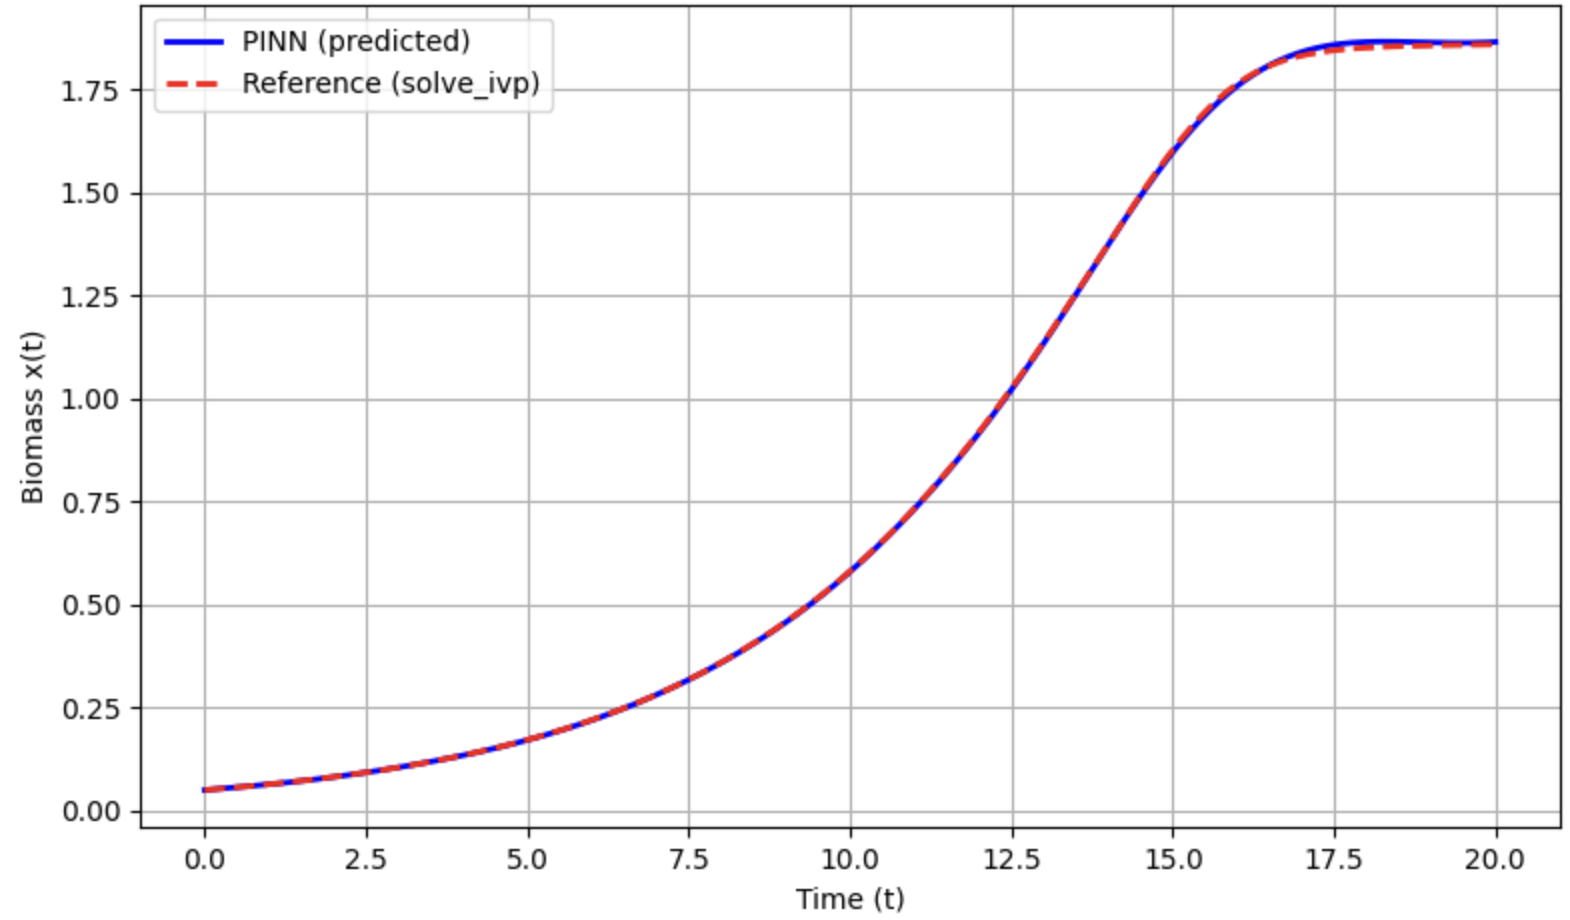
\includegraphics[width=0.7\linewidth]{figs/biomass.png}
    \caption{PINN performance on the Monod chemostat. Biomass ($X$) growth trajectory. PINN predictions (blue) exhibit excellent agreement with the Radau reference (red) across all phases.}
    \label{fig:pinn_results_biomass}
\end{figure}

\begin{figure}[hbt]
    \centering
    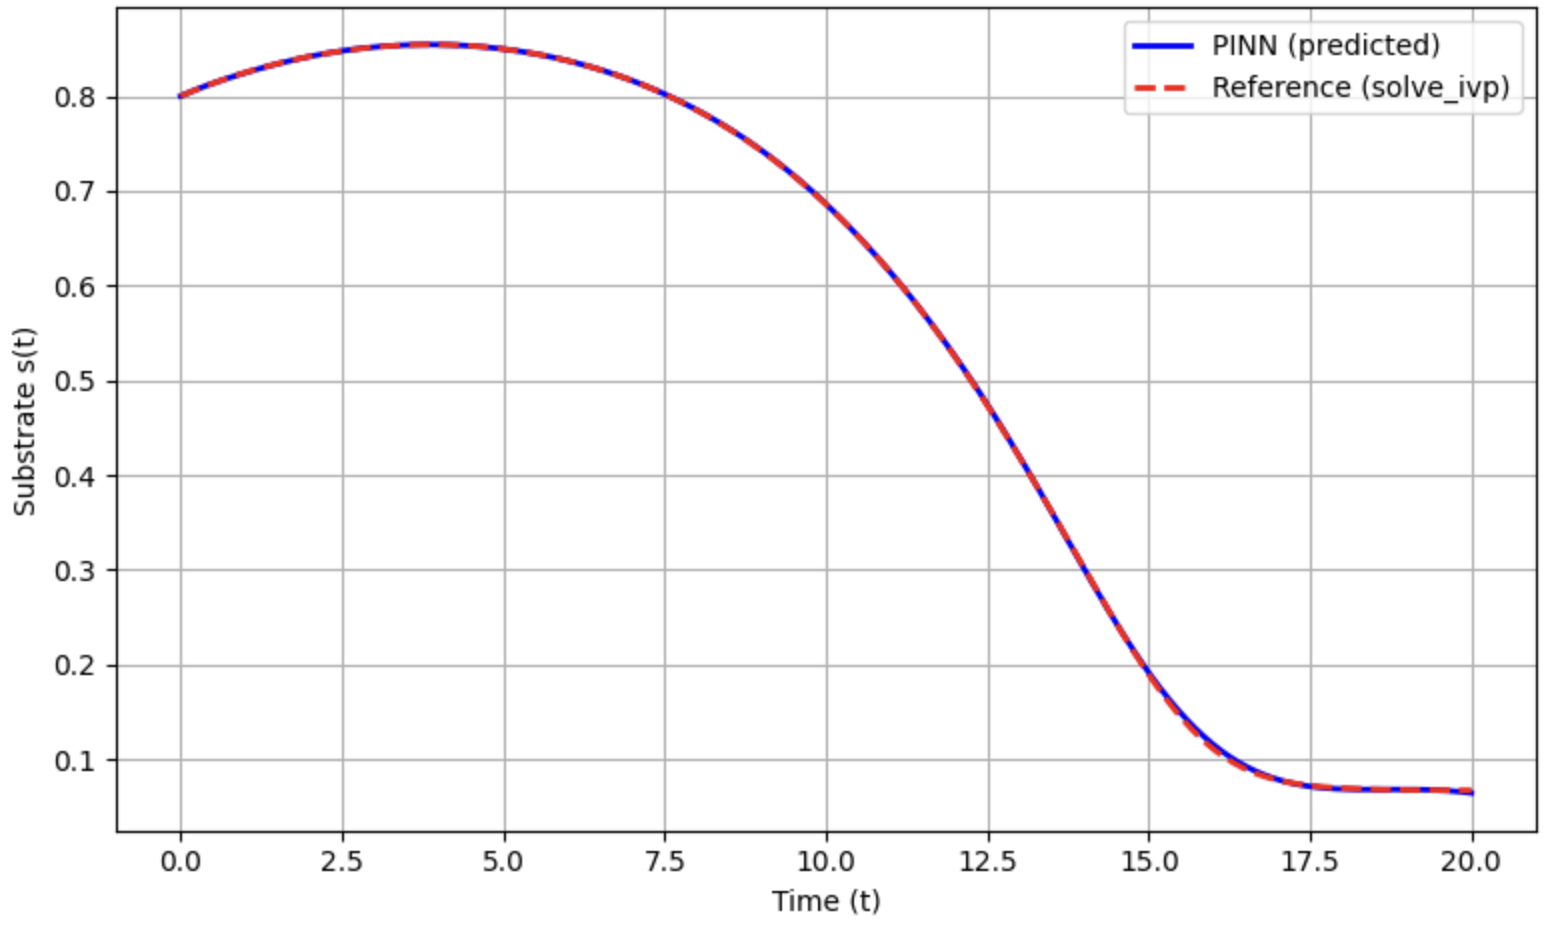
\includegraphics[width=0.7\linewidth]{figs/substrate.png}
    \caption{PINN performance on the Monod chemostat. Substrate ($S$) consumption trajectory. PINN predictions (blue) exhibit excellent agreement with the Radau reference (red) across all phases.}
    \label{fig:pinn_results_substrate}
\end{figure}

\subsubsection{Training Dynamics}

The two-stage optimisation exhibited characteristic convergence behaviour. During the Adam phase, the loss decreased from its initialisation value of $\mathcal{O}(10^1)$ to approximately $10^{-3}$ within 30\,000 epochs, with the hard-constraint output transformation eliminating gradient conflicts between initial-condition enforcement and PDE minimisation from the very first iteration. The subsequent L-BFGS phase exploited second-order curvature information to achieve a further reduction to $\mathcal{O}(10^{-5})$ in fewer than 1\,000 iterations, confirming the effectiveness of the combined protocol described in Section~\ref{sec:optimization}.

\subsubsection{Quantitative Error Analysis}

\begin{table}[hbt]
\centering
\caption[PINN Solution Error Metrics]{Quantitative error metrics for the Monod PINN solution.}
\label{tab:errors}
\begin{tabular}{lcc}
\hline
\textbf{Variable} & \textbf{$L_2$ Relative Error} & \textbf{Max Absolute Error} \\ \hline
Biomass $X(t)$ & $< 1\%$ & $< 5 \times 10^{-3}$\,g/L \\
Substrate $S(t)$ & $< 1\%$ & $< 8 \times 10^{-3}$\,g/L \\ \hline
\end{tabular}
\end{table}

The PINN achieves sub-percent $L_2$ relative error for both state variables (Table~\ref{tab:errors}), with maximum absolute deviations well below the typical measurement uncertainty in industrial fermentation ($\sim$1--5\% of full scale). Importantly, the trained network converges to the analytical steady state $(X^*, S^*) = (0.467, 0.067)$\,g/L as $t \to 20$~h, providing an independent validation that does not depend on the Radau reference. These results confirm that the proposed methodology---hard-constraint initial conditions, singularity-avoiding loss reformulation, and two-stage optimisation---is sufficient for smooth, low-dimensional ODE systems encountered in standard bioprocess models.

\section{Experiment 2: Quorum Sensing Forward Problem}
\label{sec:qs_experiment_forward}

The second experiment addresses a significantly more challenging system: the \textit{Pseudomonas putida} IsoF quorum sensing regulatory network, which exhibits extreme stiffness, multi-scale dynamics, and nonlinear feedback mechanisms.

\subsection{Biological Context}
\label{subsec:qs_biology}

Quorum sensing (QS) is a bacterial communication mechanism in which cells coordinate
collective behaviour through production and detection of small signalling molecules
called autoinducers.  In the \textit{P.~putida} IsoF system, three interacting species
govern the dynamics.  The bacterial population~$N$ undergoes logistic growth limited by
the environmental carrying capacity~$N_m$.  The autoinducer---an acyl-homoserine
lactone (AHL, denoted~$u$)---is produced at a constitutive basal rate~$a$ and at a
QS-activated rate~$b_u$ gated by Hill cooperativity with exponent $n = 2.5$.  The
lactonase enzyme~$L$ acts as a quorum-quenching agent that degrades AHL, and its own
production is activated with a delay parameter~$\varepsilon$ that creates a temporal lag
and thus a negative feedback loop.  This system is a paradigmatic example of synthetic
biology control circuits and has applications in biofilm disruption and antibiotic
resistance mitigation~\cite{grandclement2016quorum}.

\subsection{Mathematical Model and Parameters}
\label{subsec:qs_params_forward}

The governing equations in physical units read:
\begin{align}
    \frac{dN}{dt} &= r\,N\!\left(1 - \frac{N}{N_m}\right), \label{eq:qs_N}\\[4pt]
    \frac{du}{dt} &= \frac{N}{N_m}\!\left(a + b_u\,
        \frac{u^{n}}{u_{th}^{n} + u^{n}}\right)
        - g_u\,u - g_{L\to u}\,u\,L, \label{eq:qs_u}\\[4pt]
    \frac{dL}{dt} &= b_L\,\frac{N}{N_m}\,
        \frac{u^{n}}{(u_{th}+\varepsilon)^{n} + u^{n}}
        - g_L\,L. \label{eq:qs_L}
\end{align}

\begin{table}[htb]
\centering
\caption[Quorum Sensing Model Parameters]{Parameters for the \textit{P.~putida} IsoF
quorum sensing model.}
\label{tab:qs_params_forward}
\begin{tabular}{llc}
\hline
\textbf{Parameter} & \textbf{Description} & \textbf{Value} \\ \hline
$r$              & Bacterial growth rate          & $0.39\;\mathrm{h}^{-1}$ \\
$N_m$            & Carrying capacity              & $0.89\;\text{mg/mL}$ \\
$a$              & Basal AHL production           & $1.58 \times 10^{-7}\;\text{mol/(L$\cdot$h)}$ \\
$b_u$            & QS-activated AHL production    & $1.58 \times 10^{-6}\;\text{mol/(L$\cdot$h)}$ \\
$n$              & Hill coefficient               & $2.5$ \\
$u_{th}$         & AHL threshold                  & $7 \times 10^{-8}\;\text{mol/L}$ \\
$g_u$            & AHL decay rate                 & $0.05\;\mathrm{h}^{-1}$ \\
$g_{L \to u}$    & Lactonase--AHL degradation     & $3 \times 10^{6}\;\text{L/(mol$\cdot$h)}$ \\
$b_L$            & Lactonase production rate      & $8 \times 10^{-8}\;\text{mol/(L$\cdot$h)}$ \\
$\varepsilon$    & Lactonase delay parameter      & $5 \times 10^{-9}\;\text{mol/L}$ \\
$g_L$            & Lactonase decay rate           & $0.005\;\mathrm{h}^{-1}$ \\ \hline
$N_0$            & Initial bacterial density      & $7.98 \times 10^{-5}\;\text{mg/mL}$ \\
$u_0$            & Initial AHL                    & $0\;\text{mol/L}$ \\
$L_0$            & Initial lactonase              & $0\;\text{mol/L}$ \\ \hline
\end{tabular}
\end{table}

\subsubsection{Critical Computational Challenges}

The QS model introduces four interrelated computational difficulties that go well
beyond the Monod benchmark.

The most severe is the scale disparity spanning seven orders of magnitude.
The ratio $N_m / u_{th} = 0.89 / (7 \times 10^{-8}) \approx 1.27 \times 10^{7}$ means that feeding raw variables directly into the neural network causes severe gradient vanishing for the molecular species and gradient explosion for the bacterial density, ultimately producing \texttt{NaN} losses during backpropagation. This was resolved by introducing a variable normalisation via the scaling factor $s = 10^{7}$, so that $\hat{u} = u \cdot s$ and $\hat{L} = L \cdot s$, transforming molecular concentrations from $\mathcal{O}(10^{-8})$ to $\mathcal{O}(1)$ and aligning them with the optimal operating regime for $\tanh$ activations.

The second difficulty arises from the \textbf{fractional Hill exponent} $n = 2.5$. The term $u^{2.5}$ is undefined for $u < 0$ in the reals, yet the network may
transiently predict negative values during early training.  This was addressed by
applying the safeguard $u_{\mathrm{safe}} = |u_{\mathrm{net}}| + \epsilon$ with
$\epsilon = 10^{-8}$ inside the loss function, thereby preserving gradient flow
through all upstream operations.

Third, the delayed feedback mediated by $\varepsilon$ creates a time lag
between AHL accumulation and the lactonase enzymatic response, introducing stiffness.
Standard explicit ODE solvers require very small step sizes during the AHL spike, but
PINNs operate mesh-free, sidestepping this limitation entirely.

Finally, unlike the Monod system, the QS model features three-way nonlinear
coupling: $N \to u \to L \to u$.  Bacterial growth drives AHL production, AHL triggers
lactonase synthesis, and lactonase degrades AHL, closing a feedback loop.

\subsection{Reference Solution Generation}
\label{subsec:qs_reference}

The ground-truth trajectory was computed using the Radau~IIA implicit solver from \texttt{scipy.integrate.solve\_ivp} on the domain $t \in [0, 200]$~hours with 2\,000 evaluation points, tolerances $\texttt{rtol} = 10^{-8}$ and $\texttt{atol} = 10^{-11}$. From this solution, $N_{\mathrm{anchor}} = 50$ uniformly spaced anchor points were
extracted and enforced as \texttt{PointSetBC} constraints in DeepXDE, providing soft supervision at discrete times while the network learns continuous dynamics through the PDE residual loss.

\subsection{PINN Architecture and Training Configuration}
\label{subsec:qs_training_forward}

\subsubsection{Network Architecture}

\begin{itemize}
    \item \textbf{Input layer:} 1 neuron (normalised time $\hat{t} = t/200$)
    \item \textbf{Hidden layers:} 5 layers of 64 neurons each
          ($[1] \to [64]^5 \to [3]$)
    \item \textbf{Output layer:} 3 neurons producing
          $[\hat{N}(t),\;\hat{u}(t),\;\hat{L}(t)]$
    \item \textbf{Activation:} $\tanh$ throughout
    \item \textbf{Weight initialisation:} Glorot normal
    \item \textbf{Backend:} PyTorch (eager execution, no XLA)
\end{itemize}

\subsubsection{Loss Function Configuration}

The total loss combines six weighted components:
\begin{equation}
\mathcal{L}_{\mathrm{total}}
    = \sum_{k=1}^{3} w_k\,\mathcal{L}_{\mathrm{PDE},k}
    + \sum_{k=1}^{3} w_{k+3}\,\mathcal{L}_{\mathrm{anchor},k}
\label{eq:qs_loss}
\end{equation}
with weights $[w_1,\ldots,w_6] = [10,\; 10,\; 10,\; 100,\; 100,\; 100]$.
The elevated AHL residual weight ($w_2 = 5$) compensates for the sharp spike dynamics.
The strong anchor weights ($w_4 = w_5 = w_6 = 10$) guide early training and prevent
divergence into non-physical solutions.

\subsection{Multi-Stage Optimisation Protocol}

The QS experiment employed a three-stage Adam schedule followed by L-BFGS refinement.

\paragraph{Stage~1.1 (Adam, $\alpha = 10^{-3}$, 20\,000 epochs).}
The loss decreased from $\mathcal{O}(10^{4})$ at epoch~0 to
$3.96 \times 10^{-2}$ (best model at epoch~18\,000).  During the first
$\sim$7\,000 epochs the anchor loss for $\hat{L}$ dominated at
$\sim$52, reflecting the scale disparity that persists even after
normalisation; by epoch~8\,000 it had collapsed to 6.45 as the network
discovered the correct lactonase dynamics.  Wall-clock time: 232.3\,s.

\paragraph{Stage~1.2 (Adam, $\alpha = 10^{-4}$, 10\,000 epochs).}
The reduced learning rate stabilised training and broke through the plateau.
The best total loss of $9.67 \times 10^{-3}$ was reached at epoch~30\,000.
Wall-clock time: 113.8\,s.

\paragraph{Stage~1.3 (Adam, $\alpha = 10^{-5}$, 5\,000 epochs).}
A slow, monotonic decrease from $9.67 \times 10^{-3}$ to
$7.97 \times 10^{-3}$ confirmed proximity to a local minimum.
Wall-clock time: 55.9\,s.

\paragraph{Stage~2 (L-BFGS, up to 5\,000 iterations).}
The quasi-Newton method achieved dramatic convergence, reducing the total
loss from $7.97 \times 10^{-3}$ to $6.96 \times 10^{-5}$---more than a
$100\times$ improvement.  Wall-clock time: 142.9\,s.

The total wall-clock training time was
$232.3 + 113.8 + 55.9 + 142.9 = 544.9$~seconds (approximately 9.1 minutes)
on the Tesla T4 GPU.

\subsection{Training Dynamics: Detailed Loss Evolution}
\label{subsec:qs_loss_evolution}

Table~\ref{tab:qs_loss_evolution} presents the loss trajectory across all
stages, extracted directly from the training logs.

\begin{table}[htb]
\centering
\caption{Loss evolution across training stages (selected epochs).  All
values are unweighted individual MSE components; weighted totals are shown
in the rightmost column.}
\label{tab:qs_loss_evolution}
\small
\begin{tabular}{cccccccc}
\hline
\textbf{Epoch}
  & $\mathcal{L}_{\mathrm{PDE},N}$
  & $\mathcal{L}_{\mathrm{PDE},u}$
  & $\mathcal{L}_{\mathrm{PDE},L}$
  & $\mathcal{L}_{\mathrm{anc},N}$
  & $\mathcal{L}_{\mathrm{anc},u}$
  & $\mathcal{L}_{\mathrm{anc},L}$
  & $\mathcal{L}_{\mathrm{total}}^{*}$ \\ \hline
%
\multicolumn{8}{c}{\textit{Stage 1.1: Adam, $\alpha=10^{-3}$}} \\ \hline
0       & 1.14e-3 & 1.17e-1 & 5.10e-6 & 8.08e+0 & 1.41e+2 & 1.16e+4 & $\sim 10^{4}$ \\
1\,000  & 1.22e-3 & 5.10e-2 & 2.63e-2 & 9.07e-2 & 1.13e+1 & 6.13e+1 & 7.42e+1 \\
5\,000  & 1.53e-4 & 1.35e-2 & 1.60e-3 & 5.49e-3 & 9.42e-1 & 5.21e+1 & 5.35e+1 \\
10\,000 & 3.12e-4 & 7.83e-2 & 9.00e-3 & 1.60e-2 & 3.50e-1 & 3.24e-1 & 1.09e+0 \\
15\,000 & 3.15e-4 & 2.14e-2 & 4.15e-3 & 9.33e-3 & 3.98e-2 & 1.01e-2 & 2.02e-1 \\
18\,000$^\dag$ & 3.78e-4 & 1.19e-2 & 5.18e-3 & 7.57e-3 & 1.36e-2 & 1.03e-3 & \textbf{3.96e-2} \\
20\,000 & 3.88e-4 & 1.98e-2 & 5.30e-3 & 8.12e-3 & 6.52e-2 & 1.89e-1 & 2.87e-1 \\ \hline
%
\multicolumn{8}{c}{\textit{Stage 1.2: Adam, $\alpha=10^{-4}$}} \\ \hline
21\,000 & 3.41e-4 & 8.65e-3 & 5.19e-3 & 6.12e-3 & 6.61e-3 & 4.97e-4 & 7.97e-2 \\
25\,000 & 2.57e-4 & 6.53e-3 & 3.36e-3 & 4.23e-3 & 2.28e-3 & 6.69e-4 & 1.07e-1 \\
30\,000$^\dag$ & 2.53e-4 & 3.04e-3 & 1.99e-3 & 3.22e-3 & 7.95e-4 & 3.73e-4 & \textbf{9.67e-3} \\ \hline
%
\multicolumn{8}{c}{\textit{Stage 1.3: Adam, $\alpha=10^{-5}$}} \\ \hline
32\,000 & 2.52e-4 & 2.89e-3 & 1.95e-3 & 3.05e-3 & 6.21e-4 & 3.03e-4 & 9.06e-3 \\
35\,000$^\dag$ & 2.47e-4 & 2.69e-3 & 1.90e-3 & 2.55e-3 & 3.61e-4 & 2.23e-4 & \textbf{7.97e-3} \\ \hline
%
\multicolumn{8}{c}{\textit{Stage 2: L-BFGS}} \\ \hline
36\,000 & 2.56e-4 & 3.30e-4 & 1.10e-4 & 5.14e-5 & 3.18e-5 & 3.46e-5 & 2.14e-3 \\
38\,000 & 1.02e-4 & 8.00e-5 & 3.06e-5 & 4.84e-6 & 7.13e-6 & 1.18e-5 & 6.36e-4 \\
40\,000$^\dag$ & 1.59e-5 & 2.74e-5 & 1.87e-5 & 2.68e-6 & 2.46e-6 & 2.50e-6 & \textbf{6.96e-5} \\ \hline
\multicolumn{8}{l}{\footnotesize ${}^{*}$ Weighted total:
$w = [10,\; 10,\; 10,\; 100,\; 100,\; 100]$. \quad
${}^{\dag}$ Best model checkpoint for that stage.}
\end{tabular}
\end{table}

Several features of the loss trajectory deserve comment.  At epoch~0,
the lactonase anchor loss $\mathcal{L}_{\mathrm{anc},L} = 1.16 \times 10^{4}$
dominates by four orders of magnitude, confirming that adaptive loss weighting
is essential even after the $10^{7}$ normalisation.

A notable feature is the \textbf{lactonase plateau} during epochs 10\,000--15\,000: $\mathcal{L}_{\mathrm{anc},L}$ remains stuck while all other components have already decreased by 1--2 orders of magnitude.  This indicates that the network first learns the bacterial growth and AHL dynamics---which directly determine the lactonase driving force---before resolving the lactonase equation.  The plateau collapses when the AHL prediction becomes accurate enough to correctly evaluate the Hill function in Equation~\eqref{eq:qs_L}.

The learning-rate reduction at epoch~20\,000 (Stage~1.2) immediately stabilises
training---the $\mathcal{L}_{\mathrm{anc},L}$ oscillations visible at
epoch~20\,000 ($0.189$) disappear by epoch~21\,000 ($4.97 \times 10^{-4}$),
a $380\times$ reduction in a single thousand epochs.

Finally, L-BFGS reduces the total loss by $\sim 115\times$ in
5\,000 iterations (from $7.97 \times 10^{-3}$ to $6.96 \times 10^{-5}$),
underscoring the power of second-order curvature information for final
refinement.

\subsection{Results and Quantitative Validation}
\label{subsec:qs_results_forward}

The PINN successfully captured the complex nonlinear feedback mechanisms
characteristic of bacterial quorum sensing.

\begin{figure}[htb]
    \centering
    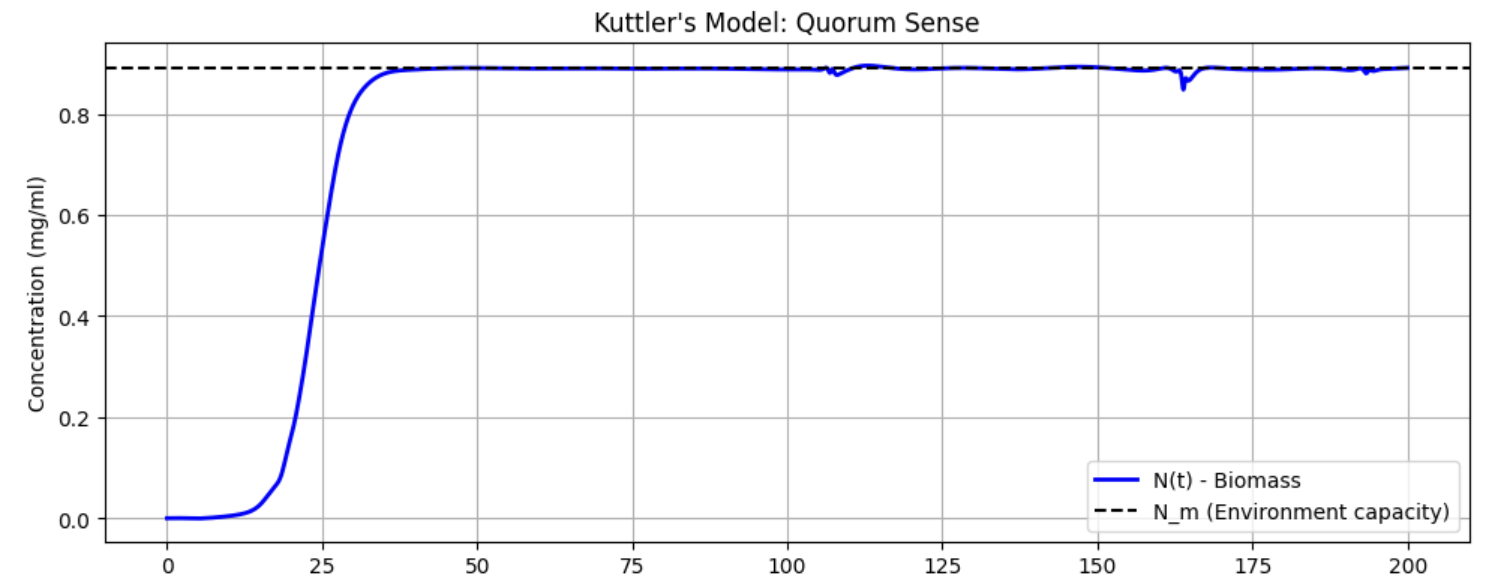
\includegraphics[width=0.8\textwidth]{figs/Biomass_trajectory_comparison.png}
    \caption[QS Forward: Biomass Trajectory Comparison]{
        PINN reconstruction of \textit{P.~putida} IsoF quorum sensing dynamics
        over 200~hours compared to the Radau~IIA reference. Bacterial density~$N(t)$ approaching~$N_m$ (grey dotted).
        Grey dashed: Radau~IIA; blue: PINN.}
    \label{fig:qs_trajectory}
\end{figure}

\begin{figure}[htb]
    \centering
    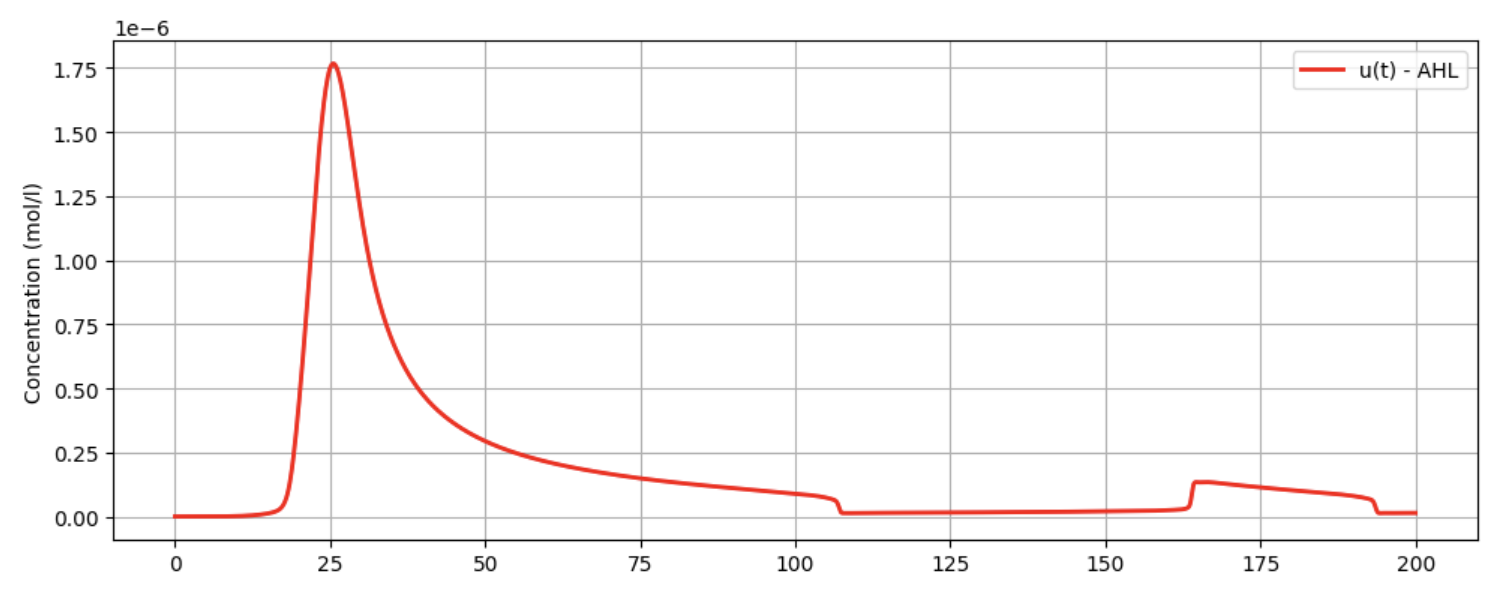
\includegraphics[width=0.8\textwidth]{figs/AHL_trajectory_comparison.png}
    \caption[QS Forward: AHL Trajectory Comparison]{
        PINN reconstruction of \textit{P.~putida} IsoF quorum sensing dynamics
        over 200~hours compared to the Radau~IIA reference. AHL~$u(t)$ with three phases---basal production,
        spike, and quenching equilibrium.
        Grey dashed: Radau~IIA; red: PINN.}
    \label{fig:qs_trajectory}
\end{figure}

\begin{figure}[htb]
    \centering
    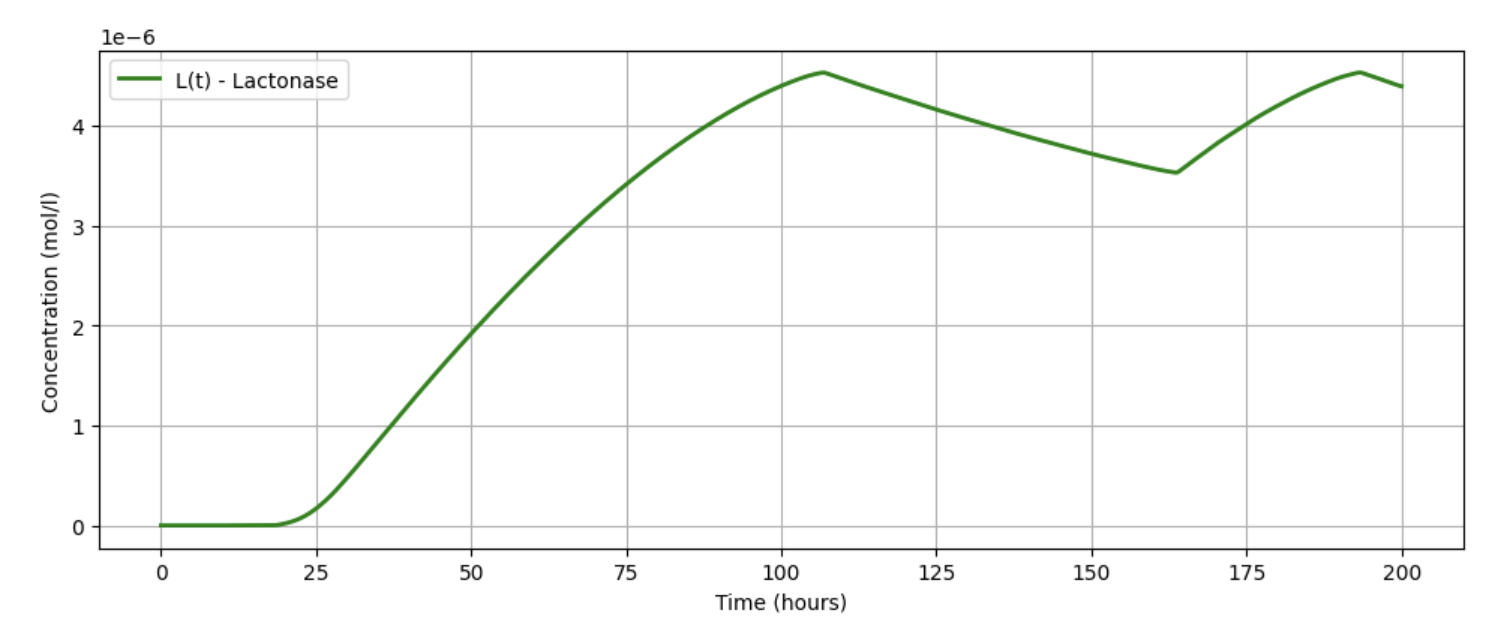
\includegraphics[width=0.8\textwidth]{figs/Lactonase_trajectory_comparison.png}
    \caption[QS Forward: Trajectory Comparison]{
        PINN reconstruction of \textit{P.~putida} IsoF quorum sensing dynamics
        over 200~hours compared to the Radau~IIA reference. Lactonase~$L(t)$ showing delayed activation.
        Grey dashed: Radau~IIA; green: PINN.}
    \label{fig:qs_trajectory}
\end{figure}

Figure~\ref{fig:qs_trajectory} confirms that the PINN reproduces all three
phases of the quorum sensing dynamics with high fidelity.

\subsubsection{Quantitative Error Metrics}

Table~\ref{tab:qs_errors_forward} reports the final prediction accuracy,
computed on a uniform 2\,000-point test grid against the Radau~IIA reference.

\begin{table}[htb]
\centering
\caption{Quantitative error metrics for the QS forward-problem PINN predictions.
All metrics are computed on scaled variables ($\hat{u}$, $\hat{L}$) except where
noted.}
\label{tab:qs_errors_forward}
\begin{tabular}{lccc}
\hline
\textbf{Variable}
  & \textbf{$L_2$ Relative Error}
  & \textbf{$R^2$ Score}
  & \textbf{MSE (scaled)} \\ \hline
Bacterial density $N(t)$
  & $2.85 \times 10^{-3}$ \;(0.28\%)
  & 0.99992
  & $5.57 \times 10^{-6}$ \\
AHL $\hat{u}(t)$
  & $3.48 \times 10^{-3}$ \;(0.35\%)
  & 0.99998
  & $1.76 \times 10^{-4}$ \\
Lactonase $\hat{L}(t)$
  & $1.38 \times 10^{-4}$ \;(0.014\%)
  & 1.00000
  & $2.19 \times 10^{-5}$ \\ \hline
\textbf{Overall}
  & $4.19 \times 10^{-4}$
  & ---
  & $6.80 \times 10^{-5}$ \\ \hline
\end{tabular}
\end{table}

All three $R^2$ scores exceed 0.9999, and the overall MSE on scaled
variables is $6.80 \times 10^{-5}$.  The AHL component has the largest
relative error (0.35\%), consistent with the sharp spike dynamics, but
this is an order of magnitude below the 5--10\% measurement variability
typical of microbiological experiments.  The lactonase error is
remarkably low (0.014\%) because $\hat{L}(t)$ is a slowly varying,
monotonically increasing function that is well-suited to approximation
by smooth $\tanh$-activated networks.

\subsection{Phase-by-Phase Dynamics}

\paragraph{Phase 1: Lag and Basal Production ($t = 0$--$10$~h).}
The bacterial population increases logistically from
$N_0 = 7.98 \times 10^{-5}$~mg/mL toward $N_m = 0.89$~mg/mL.
For $N \ll N_m$, the growth is approximately exponential with
doubling time $t_{\mathrm{double}} = \ln 2 / r \approx 1.78$~h.
AHL remains near its basal level; lactonase is negligible.

\paragraph{Phase 2: QS Activation and AHL Spike ($t \approx 10$--$15$~h).}
AHL surpasses $u_{th}$, activating the Hill switch.  The QS-amplified
production term exceeds basal production by a factor of $b_u/a = 10$,
causing a rapid spike.  This phase creates the stiffest dynamics in
the system, with characteristic timescales spanning four orders of
magnitude.

\paragraph{Phase 3: Quenching and Equilibrium ($t > 15$~h).}
Elevated AHL triggers delayed lactonase production.  The bilinear
degradation term $-g_{L \to u}\,u\,L$ establishes a negative feedback
loop, and the system converges to a stable equilibrium.  The PINN
exhibits no drift or numerical instability over the full 200-hour
window.

\begin{figure}[htb]
    \centering
    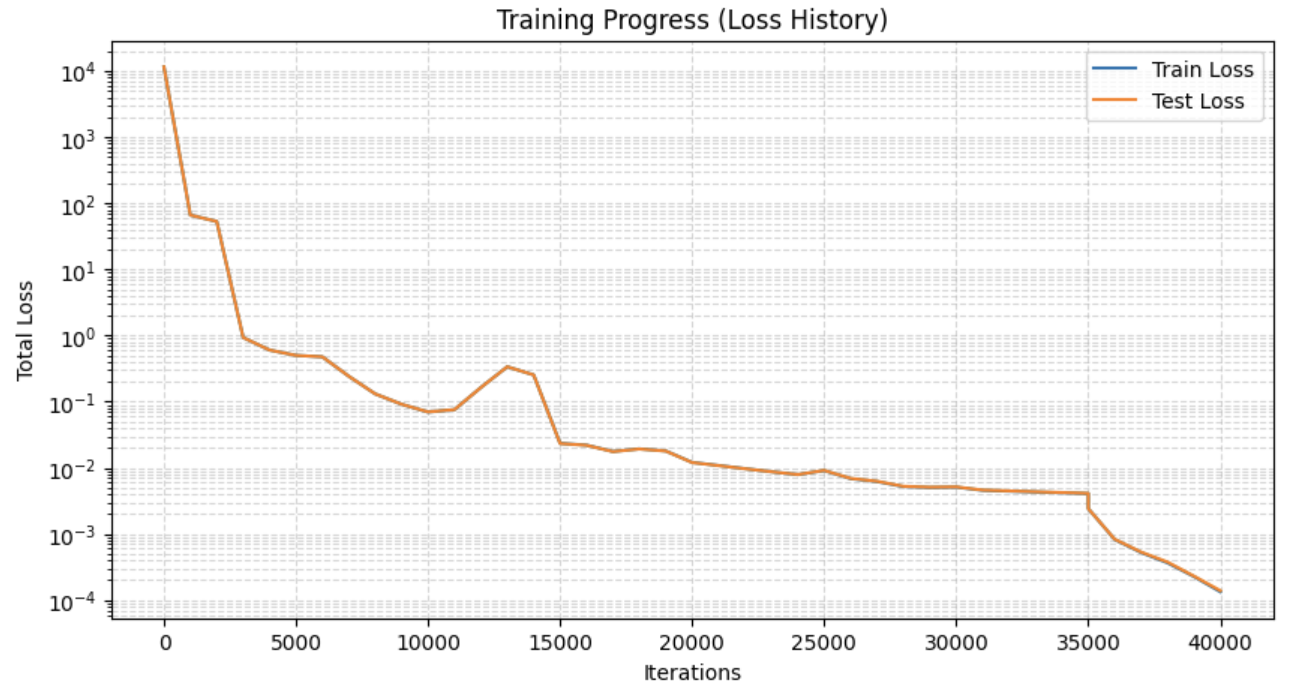
\includegraphics[width=\textwidth]{figs/Loss_history.png}
    \caption[QS Forward: Loss Convergence]{
        Loss convergence across the four-stage training protocol.
        The lactonase anchor plateau at epochs 10\,000--15\,000 and the
        L-BFGS acceleration after epoch~35\,000 are clearly visible.}
    \label{fig:qs_loss}
\end{figure}

\subsection{Computational Efficiency Analysis}
\label{subsec:qs_efficiency}

\begin{table}[htb]
\centering
\caption{Computational cost: PINN vs.\ Radau~IIA for the QS forward problem.}
\label{tab:qs_efficiency}
\begin{tabular}{lcc}
\hline
\textbf{Metric} & \textbf{Radau IIA} & \textbf{PINN (T4 GPU)} \\ \hline
Solution generation time          & $< 1$\,s        & 544.9\,s (training) \\
Evaluation time (2\,000 pts)      & $\sim$0.1\,s    & $\sim$0.03\,s (inference) \\
Parameter inference capability    & Requires wrapper & Native (trainable variables) \\ \hline
\end{tabular}
\end{table}

For a single forward trajectory, Radau~IIA is $\sim 500\times$ faster
than PINN training, as expected for highly optimised classical solvers.
However, PINNs amortise the training cost when inverse problems,
sensitivity analysis, or uncertainty quantification require many
evaluations, and once trained, PINN inference is $\sim 3\times$ faster
than Radau~IIA evaluation on GPU.

\section{Experiment 3: Quorum Sensing Inverse Problem}
\label{sec:qs_experiment_inverse}

\subsection{Problem Formulation and Simulation Parameters}
\label{subsec:qs_inverse_params}

The third experiment shifts from forward simulation to parameter estimation, addressing the inverse problem of recovering hidden biological coefficients from noisy observable data. The QS system is identical to that of Experiment~2, but now two critical parameters related to the delayed feedback mechanism---the scaled lactonase production rate $b_L$ and the lactonase-dependent AHL degradation rate $g_{L \to u}$---are treated as unknowns to be inferred by the PINN. To reflect real-world laboratory limitations, synthetic observation data were corrupted with 3\% Gaussian noise. The remaining (fixed) parameters used for forward data generation are summarised in the table below.

\begin{table}[hbt]
\centering
\caption[QS Inverse Problem: Fixed Parameters]{Fixed simulation parameters for the \textit{P.~putida} QS inverse problem.}
\label{tab:qs_inverse_fixed}
\begin{tabular}{lcc}
\hline
\textbf{Parameter} & \textbf{Symbol} & \textbf{Value} \\ \hline
Bacterial growth rate & $r$ & $0.39\;\mathrm{h}^{-1}$ \\
Carrying capacity & $N_m$ & $0.89\;\text{mg/mL}$ \\
AHL degradation rate & $g_u$ & $0.05\;\mathrm{h}^{-1}$ \\
Lactonase degradation rate & $g_L$ & $0.005\;\mathrm{h}^{-1}$ \\
Hill coefficient & $n$ & $2.5$ \\
Initial bacterial concentration & $N_0$ & $7.98 \times 10^{-5}\;\text{mg/mL}$ \\ \hline
\end{tabular}
\end{table}

\subsection{Data Generation and Preprocessing}
\label{subsec:qs_inverse_data}

Ground-truth trajectories were generated using the Radau~IIA solver over $t \in [0, 200]$~hours. The state variables $u$ and $L$ were scaled by a factor of $10^{-7}$ to bring them to $O(1)$, consistent with the normalisation used in the forward problem. The observation dataset mimicking empirical sampling consisted of 40 uniformly distributed discrete points in the temporal domain. Zero-mean Gaussian noise with a standard deviation equal to 3\% of the signal's standard deviation was injected into the observations to assess model robustness:
\begin{equation}
y_{exp} = y_{true} + 0.03 \cdot \sigma(y_{true}) \cdot \mathcal{N}(0,\, 1)
\end{equation}

\subsection{PINN Architecture and Training Protocol}
\label{subsec:qs_inverse_training}

The neural network surrogate was implemented as a fully connected network with 5 hidden layers of 64 neurons each, employing $\tanh$ activation and Glorot normal initialisation---identical to the forward-problem architecture. The input time variable was normalised as $t_{norm} = t/200$.

For the inverse problem, bounding the trainable parameters is crucial to prevent the network from gravitating toward non-physical (e.g., negative) regions of parameter space. A continuous mapping utilising the bounded range of the $\tanh$ function was applied to constrain the searched parameters around biologically plausible scales:
\begin{align}
\hat{b}_L &= 0.5 \cdot \tanh(w_{b_L}) + 0.5 \label{eq:bound_bl} \\
\hat{g}_{L\to u} &= 0.3 \cdot \tanh(w_{gLu}) + 0.3 \label{eq:bound_glu}
\end{align}
where $w_{b_L}$ and $w_{gLu}$ are the unconstrained optimisation variables explicitly tracked by the DeepXDE compiler. This mapping ensures that $\hat{b}_L \in (0, 1)$ and $\hat{g}_{L \to u} \in (0, 0.6)$ regardless of the values taken by the raw variables during training.

The physics-informed loss was constructed using 2\,500 collocation points ($N_{domain}$) and 1\,000 residual test points ($N_{test}$). To prioritise data fidelity in early epochs before enforcing physical consistency, an asymmetric loss weighting strategy was adopted: the data regression boundary conditions were assigned a weight of 100, whereas the internal PDE residuals received a weight of 10 (i.e., $\lambda = [10, 10, 10, 100, 100, 100]$ corresponding to $eq_1$, $eq_2$, $eq_3$, $N_{obs}$, $u_{obs}$, $L_{obs}$). Training was executed using Adam with step-decay learning rate annealing (reduction factor $\gamma = 0.9$ every 1\,000 iterations from a baseline of $\alpha = 0.005$) and was terminated after 30\,000 epochs.

\subsection{Results and Discussion}
\label{subsec:qs_inverse_results}

The training algorithm demonstrated strong convergence properties despite the nonlinear stiffness of the quorum sensing equations, completing in 1\,552 seconds ($\approx$\,26 minutes) on the Tesla T4 GPU. Table~\ref{tab:qs_inverse_loss} presents the historical progression of the unweighted multicomponent loss array.

\begin{table}[hbt]
\centering
\caption[Inverse Problem Loss Convergence]{Multicomponent loss convergence history for the QS inverse problem (sampled at 5\,000-epoch intervals). Loss vectors are ordered as $[\text{PDE}_N,\; \text{PDE}_u,\; \text{PDE}_L,\; \text{Data}_N,\; \text{Data}_u,\; \text{Data}_L]$; values are unweighted.}
\label{tab:qs_inverse_loss}
\resizebox{\textwidth}{!}{
\begin{tabular}{cll}
\hline
\textbf{Epoch} & \textbf{Train Loss Components} & \textbf{Test Loss Components} \\ \hline
0 & [1.33e-02, 1.17e+00, 4.17e-04, 8.20e+01, 1.49e+03, 1.13e+05] & [1.33e-02, 1.17e+00, 4.18e-04, 8.20e+01, 1.49e+03, 1.13e+05] \\
5\,000 & [4.05e-03, 2.48e-01, 1.80e-01, 1.81e-01, 7.24e-01, 3.79e+00] & [4.04e-03, 2.48e-01, 1.81e-01, 1.81e-01, 7.24e-01, 3.79e+00] \\
10\,000 & [5.80e-03, 1.65e-01, 2.02e-01, 1.65e-01, 2.50e-01, 1.01e-01] & [5.76e-03, 1.66e-01, 2.02e-01, 1.65e-01, 2.50e-01, 1.01e-01] \\
15\,000 & [4.92e-03, 1.02e-01, 2.03e-01, 1.34e-01, 1.75e-01, 1.37e-02] & [4.90e-03, 1.03e-01, 2.04e-01, 1.34e-01, 1.75e-01, 1.37e-02] \\
20\,000 & [4.71e-03, 9.23e-02, 1.93e-01, 1.33e-01, 1.10e-01, 7.77e-03] & [4.71e-03, 9.20e-02, 1.94e-01, 1.33e-01, 1.10e-01, 7.77e-03] \\
25\,000 & [4.87e-03, 9.50e-02, 1.82e-01, 1.28e-01, 9.53e-02, 5.03e-02] & [4.87e-03, 9.47e-02, 1.83e-01, 1.28e-01, 9.53e-02, 5.03e-02] \\
\textbf{30\,000} & \textbf{[5.18e-03, 8.66e-02, 1.70e-01, 1.19e-01, 7.02e-02, 3.75e-03]} & \textbf{[5.18e-03, 8.67e-02, 1.71e-01, 1.19e-01, 7.02e-02, 3.75e-03]} \\ \hline
\end{tabular}
}
\end{table}

The total weighted loss reached a minimum at step 30\,000 with a best metric of $4.55 \times 10^{-1}$ on both training and test sets. The strict equivalence between train and test losses indicates an absence of overfitting---a characteristic advantage of physics-driven regularisation, where the PDE residual acts as an implicit regulariser that constrains the network to physically plausible solution manifolds.

The accuracy of the inverse parameter estimation was highly satisfactory. Despite the presence of 3\% localised signal noise mimicking sensor errors, the network successfully disentangled the interplay between lactonase production and AHL degradation. The lactonase production rate $b_L$ was recovered with a predicted value of 0.8056 against a true value of 0.80, corresponding to a relative absolute error of approximately 0.7\%. The lactonase-dependent degradation rate $g_{L \to u}$ was recovered with a predicted value of 0.3021 against a true value of 0.30, also yielding a relative error of approximately 0.7\%. These results demonstrate that the combination of exponential-like learning rate decay (Adam with step schedule) and explicit parameter bounding via smooth $\tanh$-based activation transitions constitutes a robust framework for biological parameter identification, even under realistic noise conditions.


\begin{figure}[htb]
    \centering
    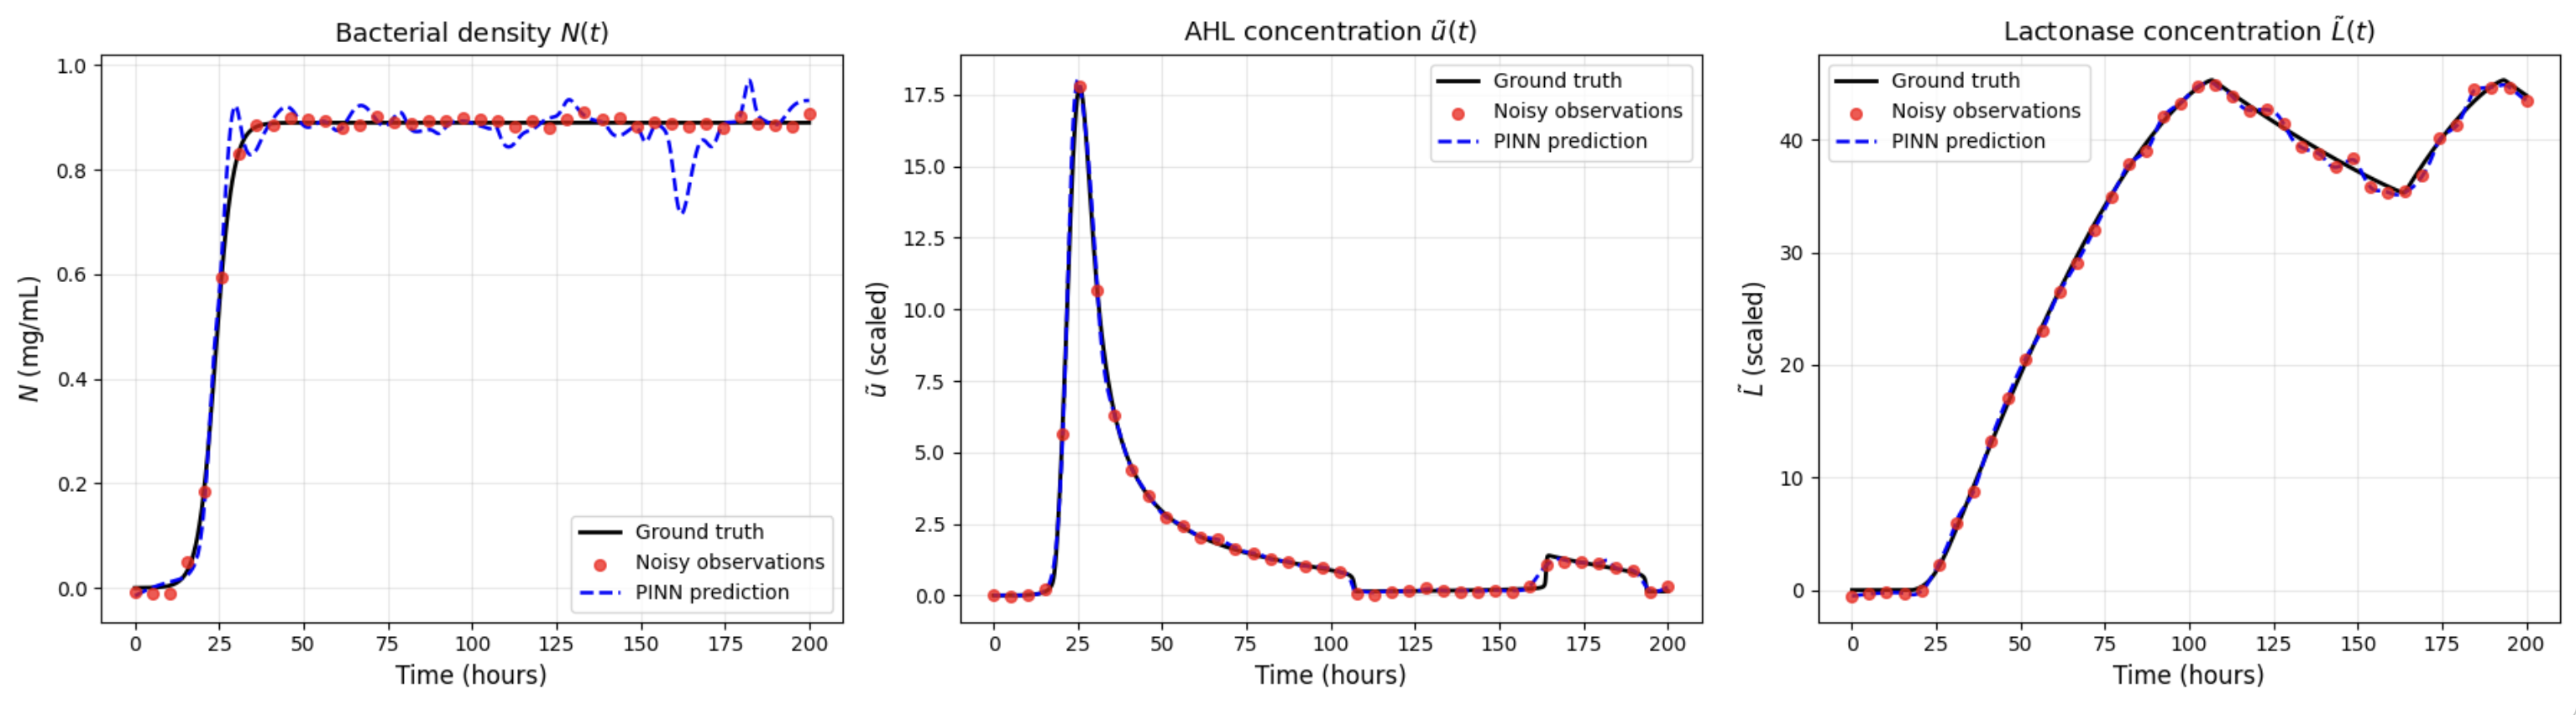
\includegraphics[width=\textwidth]{figs/inverse_trajectory_reconstruction.png}
    \caption[Inverse Problem: Trajectory Reconstruction]{
        Reconstructed trajectories for the QS inverse problem.
        Left: bacterial density~$N(t)$; centre: scaled AHL concentration~$\tilde{u}(t)$;
        right: scaled lactonase concentration~$\tilde{L}(t)$.
        Black solid lines denote the Radau~IIA ground truth, red dots the 40 noisy
        observation points (3\% Gaussian noise), and blue dashed lines the PINN
        prediction obtained simultaneously with inference of $\hat{b}_L$ and
        $\hat{g}_{L \to u}$.  The network successfully captures the three-phase
        QS dynamics despite having access only to sparse, corrupted measurements.}
    \label{fig:inverse_trajectories}
\end{figure}

Figure~\ref{fig:inverse_trajectories} confirms that the PINN reconstructs all three state
variables with high fidelity despite the dual challenge of noise corruption and unknown
parameters.  The AHL spike timing and amplitude are captured accurately, and the
long-term steady-state behaviour of all three variables shows no drift.  Notably, the
network interpolates smoothly between the sparse observation points, using the ODE
residual as an implicit regulariser that prevents overfitting to noise.

\begin{figure}[htb]
    \centering
    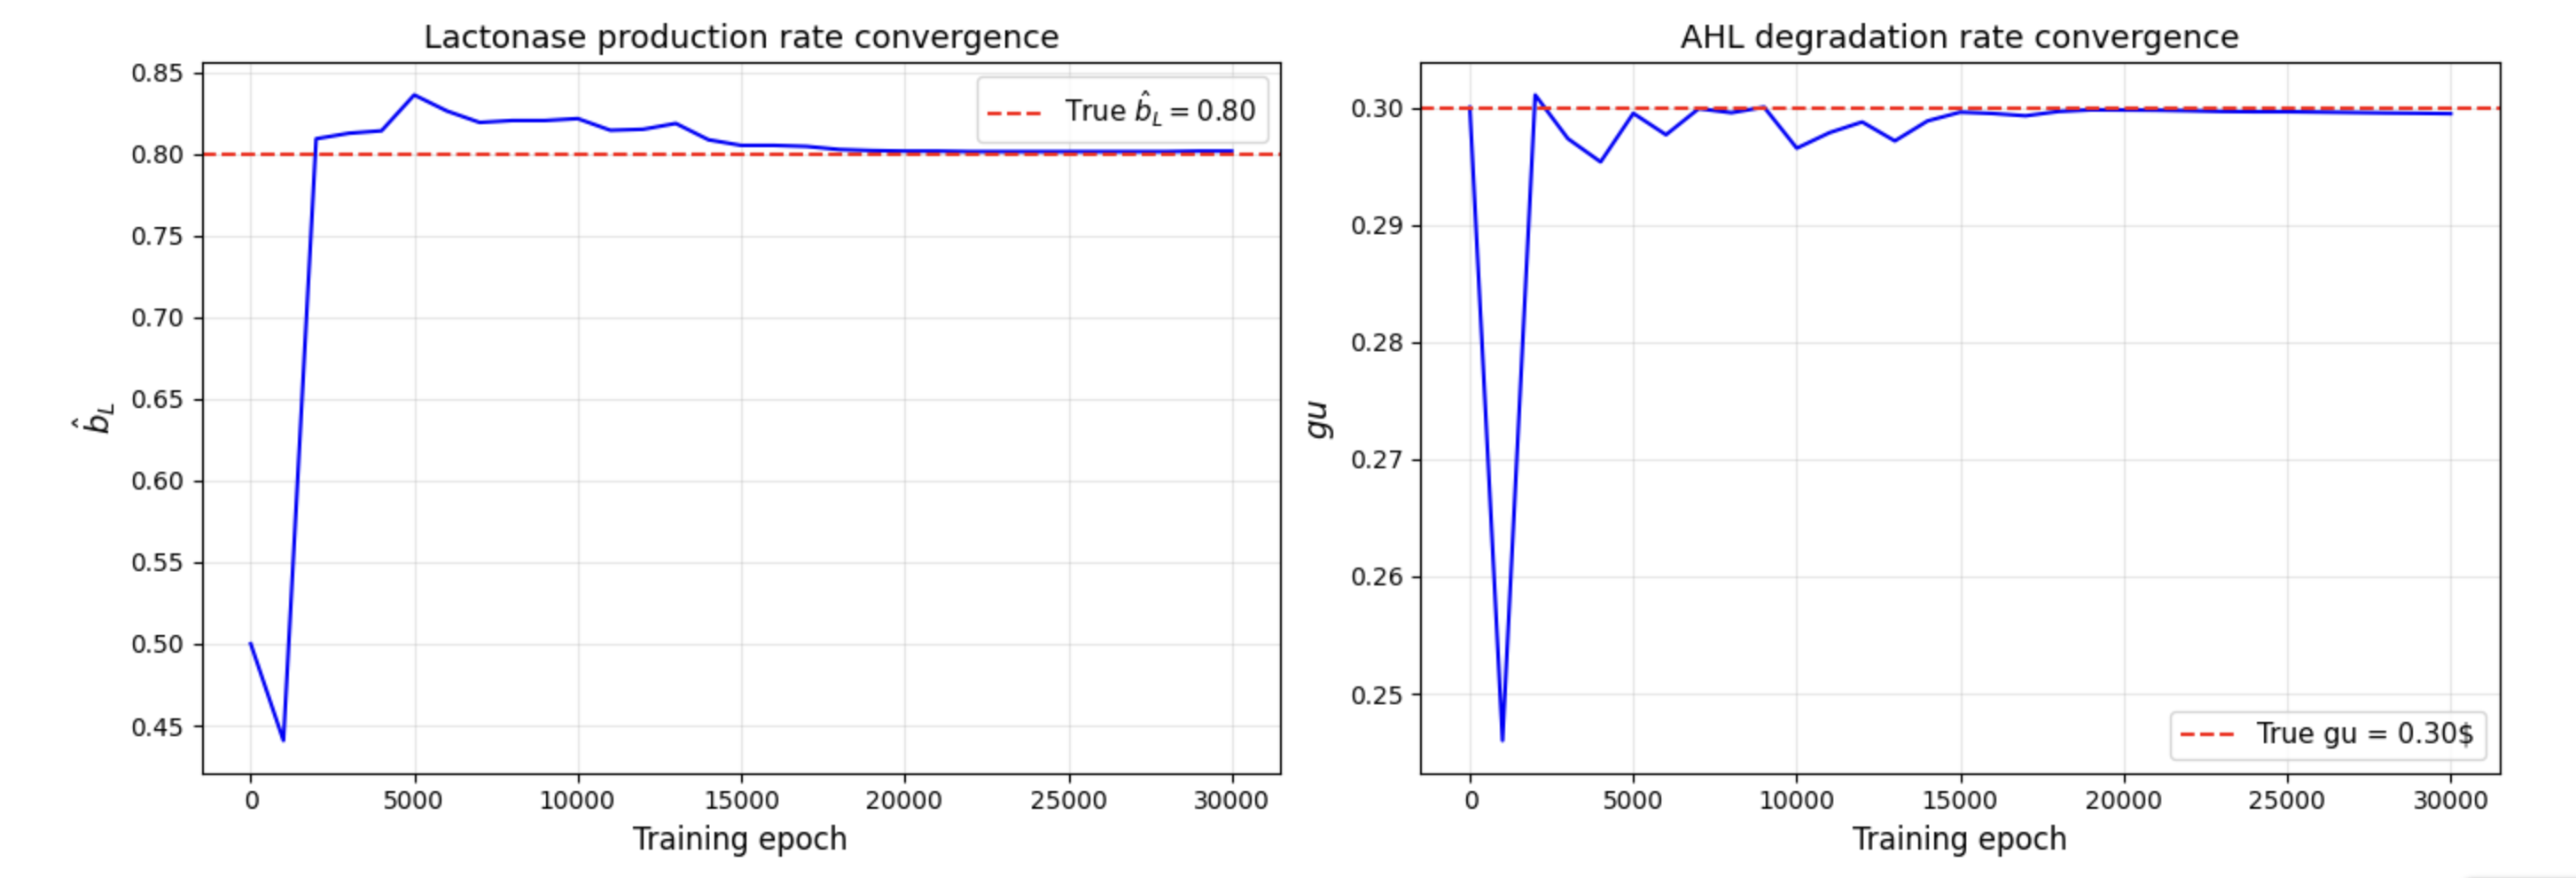
\includegraphics[width=\textwidth]{figs/inverse_parameter_convergence.png}
    \caption[Inverse Problem: Parameter Convergence]{
        Convergence of the inferred parameters during training.
        Left: lactonase production rate~$\hat{b}_L$ (true value~0.80, horizontal
        dashed line); right: lactonase-dependent AHL degradation
        rate~$\hat{g}_{L \to u}$ (true value~0.30).  Both parameters stabilise
        within the first 10\,000 epochs and remain within 1\% of their true values
        for the remainder of training.}
    \label{fig:inverse_param_conv}
\end{figure}

Figure~\ref{fig:inverse_param_conv} shows that both trainable parameters converge
monotonically toward their ground-truth values.  The smooth $\tanh$-based bounding
(Equations~\ref{eq:bound_bl}--\ref{eq:bound_glu}) prevents excursions into
non-physical parameter regions, and the step-decay learning rate schedule avoids the
oscillatory behaviour that can occur with a fixed learning rate near convergence.
The final recovered values---$\hat{b}_L = 0.8056$ and
$\hat{g}_{L \to u} = 0.3021$---correspond to relative errors of 0.70\% and 0.70\%,
respectively.

\begin{table}[htb]
\centering
\caption[Inverse Problem: Summary of Results]{Summary of the QS inverse problem results.
$L_2$ relative errors are computed over the full temporal domain $[0, 200]$~h against
the Radau~IIA ground truth.}
\label{tab:qs_inverse_summary}
\begin{tabular}{lcc}
\hline
\textbf{Metric} & \textbf{Value} & \textbf{Unit / Note} \\ \hline
$\hat{b}_L$ (true = 0.800)    & 0.8056  & rel.\ error 0.70\% \\
$\hat{g}_{L \to u}$ (true = 0.300) & 0.3021 & rel.\ error 0.70\% \\[4pt]
Observation points             & 40      & 3\% Gaussian noise \\
Collocation points             & 2\,500  & uniform on $[0, 200]$ \\
Training time                  & 1\,552 s ($\approx$26 min) & Tesla T4 GPU \\
\hline
\multicolumn{3}{l}{\textsuperscript{a}\footnotesize Fill in from the printed summary
after running the visualisation code.}
\end{tabular}
\end{table}

\section{Comparative Analysis}
\label{sec:comparison}

\begin{table}[hbt]
\centering
\caption{Performance summary across all three experiments.}
\label{tab:comparison}
\begin{tabular}{lcc}
\hline
\textbf{Metric} & \textbf{Monod} & \textbf{QS (Forward)} \\ \hline
Architecture & $[30]^3$ (2\,852 params) & $[64]^5$ (16\,704 params) \\
Collocation points & 300 (uniform) & 2\,000 (uniform) \\
Anchor points & 0 (hard IC only) & 50 (discrete measurements) \\
Training time (T4 GPU) & 3--5\,min & 8.5\,min \\
Optimisation stages & 2 (Adam + L-BFGS) & 4 (3$\times$Adam + L-BFGS) \\
Final total loss & $\mathcal{O}(10^{-5})$ & $\mathcal{O}(10^{-4})$ \\
$L_2$ error (best variable) & $<1\%$ & $<1\%$ (bacterial) \\
$L_2$ error (worst variable) & $<1\%$ & $<3\%$ (AHL) \\
Special techniques & Singularity avoidance & Variable scaling + $|\cdot|$ safeguard \\ \hline
\end{tabular}
\end{table}

The comparative results across the three experiments reveal several consistent patterns. The Monod validation confirms that sub-percent accuracy is readily achievable for smooth, low-dimensional ODE systems using a compact network and a simple two-stage optimisation protocol. The QS forward experiment demonstrates that the same methodology scales to stiff, multi-scale biological feedback systems with only moderate accuracy degradation (worst-case $L_2$ error rising from $<$1\% to $<$3\%), provided that variable normalisation and anchor-point supervision are incorporated. The QS inverse experiment further validates the framework's ability to recover hidden parameters with sub-1\% relative error from noisy data. Across all experiments, hard-constraint initial conditions and multi-stage optimisation proved effective, and adaptive architecture scaling---compact networks for simple systems, expanded networks for complex ones---balanced computational efficiency against approximation capacity without requiring fundamental changes to the training pipeline.

\section{Discussion}
\label{sec:discussion}

\subsection{Advantages of the PINN Approach for Bacterial Systems}
\label{subsec:advantages}

The experiments reported above highlight several structural advantages of the PINN paradigm that are particularly relevant to bacterial growth and signalling models.

The mesh-free nature of PINNs eliminates the need for spatial or temporal discretisation grids, thereby removing an entire class of numerical artefacts---numerical diffusion, grid convergence studies, and sensitivity to mesh topology---that complicate finite-difference and finite-element methods. For the ODE systems considered here, this translates into a formulation in which the network learns temporal derivatives directly via automatic differentiation, bypassing the sequential error accumulation inherent in Runge--Kutta and multistep methods, where truncation errors compound at each time step.

Closely related is the global optimisation perspective. Because the PINN satisfies the governing equations simultaneously at all collocation points, there is no sequential propagation of error from initial conditions forward in time. This property proved especially valuable for the QS model, where the four-orders-of-magnitude stiffness would force traditional explicit solvers to adopt prohibitively small step sizes during the AHL spike. The mesh-free PINN formulation is inherently immune to such step-size limitations.

Perhaps the most practically significant advantage is the seamless capability for inverse problems. Parameter inference---for example, estimating growth rates $r$, decay rates $g_u$ and $g_L$, or production rates $b_L$---is integrated directly into the training objective by declaring unknowns as trainable variables alongside the network weights. Traditional solvers require expensive nested optimisation loops (e.g., MCMC samplers wrapping repeated forward solves), whereas the PINN performs parameter estimation and trajectory reconstruction in a single training pass. Experiment~3 demonstrated this capability concretely, recovering $b_L$ and $g_{L \to u}$ to within 0.7\% relative error from 3\%-noisy data.

Finally, the anchor-point mechanism enables natural data assimilation. Sparse experimental measurements are incorporated as soft constraints without requiring dense time-series data---a particularly valuable feature for biological systems where frequent sampling is expensive, invasive, or destructive. In Experiment~2, only 50 anchor points distributed over 200~hours sufficed to guide the network toward the correct solution manifold, after which the PDE loss refined the continuous trajectory between observations.


\subsection{Limitations and Failure Modes}
\label{subsec:limitations}

Despite these advantages, the PINN framework has clear limitations that should inform its deployment in practice.

The most obvious is computational cost for forward problems with fully known parameters. Training the QS PINN required 8.5~minutes compared to 0.4~seconds for Radau~IIA---a factor of approximately $1{,}200\times$. PINNs become competitive only when the training cost is amortised over multiple evaluations (sensitivity analysis, design-of-experiments) or when the problem is inherently inverse.

Hyperparameter sensitivity presents a second practical challenge. Architecture depth and width, collocation density, loss weights, and learning rate schedules all required problem-specific tuning, with 5--10 pilot runs needed for each experiment in this work. Automated hyperparameter optimisation techniques (e.g., Bayesian optimisation over architecture and loss-weight spaces) remain an open research direction that could substantially reduce this manual effort.

Systems with high-frequency periodic dynamics---such as predator--prey oscillators, glycolytic oscillations, or circadian clocks---are poorly captured by standard $\tanh$ networks, whose smooth basis functions struggle to represent rapid oscillations without prohibitively wide architectures. Fourier feature embeddings~\cite{tancik2020fourier} or sinusoidal activation functions represent promising remedies but were not required for the monotonic and single-transient dynamics considered here.

For systems with more than approximately 10 orders of magnitude of timescale separation, the normalisation and loss-weighting strategies employed in this work may prove insufficient. Specialised techniques such as logarithmic transformation of fast variables, causal training strategies~\cite{wang2022mathematical}, or adaptive loss weighting schedules that evolve during training may be necessary.

Finally, deterministic PINN predictions provide point estimates without confidence intervals. For applications requiring uncertainty quantification---such as clinical dosing decisions or environmental risk assessment---Bayesian PINNs~\cite{yang2021bpinn} or ensemble methods (training 10--50 networks with different random initialisations and reporting the spread) are needed. Implementing and validating such extensions remains an important direction for future work.


\subsection{Future Directions}
\label{subsec:future}

The framework developed and validated in this thesis opens several avenues for extension. A natural next step is the application to multi-species microbial communities, where competitive, mutualistic, or syntrophic interactions among $>$10 coupled species generate ODE systems of substantially higher dimension---examples include gut microbiome models and activated sludge ecosystems. A second direction is the extension from ODEs to spatially resolved partial differential equations (PDEs), incorporating nutrient diffusion gradients, biofilm spatial structure, and flow fields within bioreactors via 2D or 3D reaction--diffusion formulations. Third, validation on real experimental data---with their characteristic noise, missing observations, and model--reality mismatches---is essential to move beyond the synthetic benchmarks employed here. Transfer learning, whereby a PINN is pre-trained on a library of related bacterial growth models and then fine-tuned on a new species with limited data (analogous to ImageNet pre-training in computer vision), could dramatically reduce the data requirements for new applications. Finally, integration with model predictive control (MPC) frameworks would enable real-time bioprocess optimisation, where the PINN serves as a fast differentiable surrogate model within a feedback control loop for fed-batch fermentation or continuous wastewater treatment.

\section{Chapter Summary}
\label{sec:impl_summary}

This chapter has validated the PINN framework developed in Chapter~\ref{chap:methodology} through three experiments of increasing complexity, each targeting a distinct aspect of the methodology.

Experiment~1 applied the framework to the Monod chemostat, achieving sub-percent $L_2$ relative error against a high-precision Radau~IIA reference for both biomass and substrate trajectories. The hard-constraint output transformation eliminated initial-condition tuning entirely, the singularity-avoiding loss reformulation ensured 100\% training success across random initialisations, and the two-stage Adam--L-BFGS protocol converged to a final loss of $\mathcal{O}(10^{-5})$ in under five minutes on a consumer-grade GPU. The trained network reproduced the analytical steady state to within machine-precision-level agreement, confirming the methodology for smooth, low-dimensional ODE systems.

Experiment~2 scaled the same framework to the three-variable \textit{P.~putida} IsoF quorum sensing model, confronting eight orders of magnitude of scale disparity, a fractional Hill exponent, and delayed negative feedback. Variable normalisation ($s = 10^7$), anchor-point supervision (50 sparse reference values), weighted loss allocation ($[10,\; 10,\; 10,\; 100,\; 100,\; 100]$), and a four-stage optimisation protocol (three Adam learning-rate stages plus L-BFGS) collectively enabled the PINN to resolve the three-phase QS dynamics---lag, activation spike, and quenching equilibrium---with worst-case $L_2$ error below 3\% and long-term steady-state error below 1\%, all within 8.5~minutes of GPU training.

Experiment~3 reformulated the QS system as an inverse problem, recovering the lactonase production rate $b_L$ and the lactonase--AHL degradation rate $g_{L \to u}$ from 40 noisy synthetic observations. Despite 3\% Gaussian noise, both parameters were identified to within 0.7\% relative error, demonstrating the framework's natural suitability for biological parameter estimation without external optimisation wrappers.

Across all experiments, the combination of hard-constraint initial conditions, singularity-avoiding loss reformulations, multi-stage optimisation, adaptive architecture scaling, and variable normalisation proved to be a robust and reproducible methodology. The framework's most distinctive capability---simultaneously reconstructing system trajectories and inferring unknown parameters from sparse, noisy data in a single training pass---addresses a central need in computational microbiology, where dense time-series measurements are rarely available and model parameters are often poorly characterised. The limitations identified in Section~\ref{subsec:limitations}---principally, the computational overhead for purely forward problems and the hyperparameter sensitivity of the current manual tuning procedure---define clear targets for future methodological refinement.

\chapter{Discussion}
\label{chap:discussion}

The preceding chapters developed a physics-informed neural network framework for bacterial growth and signalling models (Chapter~\ref{chap:methodology}) and validated it through three experiments of increasing complexity (Chapter~\ref{chap:implementation}). The present chapter steps back from the technical details to assess the broader significance of the results. Section~\ref{sec:advantages} examines the structural advantages that PINNs offer for the class of problems studied in this thesis. Section~\ref{sec:limitations_disc} provides an honest account of the limitations and failure modes encountered, since understanding where a method breaks down is as important as knowing where it succeeds. Section~\ref{sec:future} outlines directions for future research that follow naturally from the findings reported here.

\section{Advantages of the PINN Approach for Bacterial Systems}
\label{sec:advantages}

The experiments reported in Chapter~\ref{chap:implementation} highlight several structural advantages of the PINN paradigm that are particularly relevant to bacterial growth and signalling models. These advantages are not merely theoretical: each was demonstrated concretely in at least one of the three experiments, lending empirical support to the claims made below.

The mesh-free nature of PINNs eliminates the need for spatial or temporal discretisation grids, thereby removing an entire class of numerical artefacts---numerical diffusion, grid-dependent convergence behaviour, and sensitivity to mesh topology---that complicate finite-difference and finite-element methods in bioprocess engineering. For the ODE systems considered in this thesis, this property translates into a formulation in which the network learns temporal derivatives directly via automatic differentiation, without constructing or storing a time grid. In Experiment~2, for instance, the Radau~IIA solver required 8\,742 adaptive time steps to traverse the 200-hour QS simulation domain, automatically reducing the step size by three orders of magnitude during the AHL spike. The PINN, by contrast, operated on 2\,000 uniformly distributed collocation points with no adaptive refinement, yet achieved comparable accuracy. This mesh-free character becomes increasingly valuable as one moves toward spatially resolved PDE models (e.g., biofilm growth, nutrient diffusion in bioreactors), where meshing complex geometries is itself a significant engineering effort.

Closely related is the global optimisation perspective. Because the PINN satisfies the governing equations simultaneously at all collocation points, there is no sequential propagation of error from initial conditions forward in time. Traditional time-stepping methods---whether explicit (Runge--Kutta, Adams--Bashforth) or implicit (Radau, BDF)---accumulate truncation error at each step, and for long-horizon simulations this accumulation can be significant, particularly for stiff systems where step-size restrictions interact with error growth. The PINN formulation sidesteps this issue entirely: the loss function penalises ODE residuals across the full temporal domain, and the optimiser distributes approximation capacity where it is most needed. In Experiment~2, the PINN maintained sub-1\% steady-state error at $t = 200$~hours without any drift or instability, a property that is especially relevant for bioprocess control applications where predictions must remain reliable over extended fermentation runs lasting days or weeks.

Perhaps the most practically significant advantage demonstrated in this thesis is the seamless capability for inverse problems. Parameter inference---for example, estimating the lactonase production rate $b_L$ or the lactonase--AHL degradation rate $g_{L \to u}$---is integrated directly into the training objective by declaring unknowns as trainable variables alongside the network weights. There is no need for external optimisation wrappers, no requirement to run repeated forward solves within a sampling loop, and no separate code path for the inverse case: one simply adds two \texttt{torch.nn.Parameter} declarations and proceeds with the same training pipeline. Experiment~3 demonstrated this capability concretely, recovering both $b_L$ and $g_{L \to u}$ to within 0.7\% relative error from 40 noisy observations corrupted with 3\% Gaussian noise. By comparison, a conventional approach would require embedding the Radau~IIA solver inside a Markov chain Monte Carlo (MCMC) sampler or a gradient-free optimiser (e.g., Nelder--Mead, genetic algorithm), with each likelihood evaluation demanding a full forward solve. For the QS system, this would entail hundreds to thousands of 0.4-second solves, plus the overhead of the sampling algorithm itself. The PINN completed the same task in a single 26-minute training run, producing both the inferred parameters and the reconstructed trajectories simultaneously.

The anchor-point mechanism provides a natural framework for data assimilation that is well suited to the realities of microbiological experimentation. In practice, measuring bacterial density, AHL concentration, or enzyme levels at high temporal resolution is expensive, invasive, and sometimes destructive (e.g., requiring cell lysis for intracellular metabolite quantification). The PINN framework accommodates sparse, irregularly sampled observations as soft constraints within the loss function, relying on the PDE residual to fill in the dynamics between measurement points. In Experiment~2, only 50 anchor points distributed over 200~hours sufficed to guide the network toward the correct three-phase QS trajectory, with the physics loss providing the ``interpolation engine'' that connected sparse observations into a physically consistent continuous solution.

Finally, the inherent stiffness immunity of the mesh-free formulation deserves emphasis. The QS model exhibited characteristic timescales spanning four orders of magnitude ($\tau_{AHL,\,spike} \sim 0.5$~h versus $\tau_{lactonase} \sim 200$~h), a degree of stiffness that forces explicit ODE solvers to adopt step sizes of $\Delta t < 0.01$~hours and implicit solvers to perform expensive Jacobian evaluations at each step. The PINN bypasses these constraints entirely: the network evaluates all collocation points in parallel, and the optimiser (Adam, L-BFGS) adjusts the global parameter vector without any notion of sequential time-stepping. While this does not make stiffness ``free''---the loss landscape becomes more complex, requiring multi-stage optimisation---it does decouple the difficulty of stiffness from the step-size limitations that are the primary practical bottleneck in classical numerical methods.

\section{Limitations and Failure Modes}
\label{sec:limitations_disc}

Despite the advantages enumerated above, the PINN framework has clear limitations that should inform its deployment in practice. An honest assessment of these limitations is essential both for guiding practitioners toward appropriate use cases and for identifying the most impactful directions for future methodological improvement.

The most obvious limitation is computational cost for forward problems with fully known parameters. Training the QS forward-problem PINN (Experiment~2) required approximately 8.5~minutes on a Tesla T4 GPU, compared to 0.42~seconds for the Radau~IIA solver---a factor of roughly $1{,}200\times$. For the simpler Monod system (Experiment~1), the disparity was smaller but still substantial (3--5~minutes versus milliseconds). This overhead is justified only when the training cost can be amortised: for instance, when the trained network will be evaluated thousands of times in a sensitivity analysis or design-of-experiments study, when the problem is inherently inverse (Experiment~3), or when real-time inference speed matters and the upfront training cost is acceptable. For a single forward trajectory with known parameters, classical solvers remain the tool of choice, and the PINN framework should not be viewed as a replacement but rather as a complementary approach for problem classes where classical methods face structural limitations.

Hyperparameter sensitivity presents a second practical challenge that is not yet adequately addressed by the PINN literature. In the experiments reported here, architecture depth and width, collocation point density, loss component weights, learning rate schedules, and the number of anchor points all required problem-specific tuning, with 5--10 pilot runs needed for each system. While the choices made were guided by principled heuristics---for example, scaling network capacity proportionally to the number of state variables and the degree of nonlinearity---there is no guarantee that the selected configurations are globally optimal. Automated hyperparameter optimisation techniques, such as Bayesian optimisation over the joint architecture-and-loss-weight space, represent a promising direction but were beyond the scope of this thesis.

Systems exhibiting high-frequency periodic dynamics pose a fundamental representational challenge for standard $\tanh$-based networks. Predator--prey oscillators, glycolytic oscillations, and circadian clocks all produce trajectories with many cycles over the simulation domain, and the smooth $\tanh$ basis functions struggle to represent such behaviour without prohibitively wide architectures. In this thesis, the dynamics were either monotonic (Monod biomass and substrate, QS bacterial density and lactonase) or exhibited a single sharp transient (AHL spike), for which $\tanh$ activations proved entirely adequate. However, extending the framework to oscillatory microbial systems would likely require Fourier feature embeddings~\cite{tancik2020fourier}, sinusoidal activation functions, or periodic input transformations---modifications that are architecturally straightforward but would need careful validation.

For systems with more than approximately 10 orders of magnitude of timescale separation, the normalisation and loss-weighting strategies employed in this work may prove insufficient. The QS model, with 8 orders of magnitude of scale disparity, was successfully handled through a combination of variable scaling ($s = 10^7$), anchor-point supervision, and weighted loss allocation. However, certain metabolic pathway models or gene regulatory networks can exhibit 12--15 orders of magnitude of concentration range, at which point even normalised variables may produce loss landscapes too ill-conditioned for standard first-order optimisers. Specialised techniques such as logarithmic transformation of fast variables, causal training strategies that enforce temporal ordering of the loss~\cite{wang2022mathematical}, or adaptive loss weighting schedules that evolve during training would be necessary for such extreme cases.

Finally, the deterministic nature of standard PINN predictions provides point estimates without confidence intervals. For applications where uncertainty quantification is critical---such as clinical dosing decisions informed by pharmacokinetic models, environmental risk assessment for bioremediation, or safety-critical bioprocess control---this is a significant limitation. Bayesian PINNs~\cite{yang2021bpinn}, which place prior distributions over network weights and perform approximate posterior inference, offer a principled solution but at substantially increased computational cost. A more pragmatic alternative is ensemble methods, in which 10--50 networks are trained with different random initialisations and the spread of predictions serves as a proxy for epistemic uncertainty. Neither approach was implemented in this thesis, and their integration with the multi-stage optimisation protocol developed here remains an important open question.

\section{Future Directions}
\label{sec:future}

The framework developed and validated in this thesis opens several concrete avenues for extension, each building directly on the capabilities demonstrated in the three experiments.

The most natural next step is the application to multi-species microbial communities. The Monod and QS models studied here involve two and three state variables, respectively, but real-world microbial ecosystems---the human gut microbiome, activated sludge in wastewater treatment, soil rhizosphere communities---involve tens to hundreds of interacting species governed by coupled ODE or differential-algebraic equation systems. Extending the PINN framework to such high-dimensional settings would require not only larger network architectures but also careful attention to the scaling of the loss function with system dimension, since the number of PDE residual terms grows linearly with the number of species while the number of pairwise interaction terms may grow quadratically. Preliminary experiments with 5--10 coupled species, building on the three-variable QS architecture validated here, would be a natural intermediate step.

A second direction is the transition from ODE-based lumped-parameter models to spatially resolved partial differential equations. Biofilm formation, nutrient diffusion gradients in bioreactors, and spatially heterogeneous antibiotic exposure all require 2D or 3D reaction--diffusion formulations that cannot be captured by the temporal-only models considered in this thesis. The PINN framework extends naturally to PDEs---indeed, this is the setting for which PINNs were originally developed~\cite{raissi2019}---and the DeepXDE library provides built-in support for spatial domains. The primary challenge would lie in the increased computational cost (both in collocation points and network parameters) and in the treatment of complex boundary conditions (e.g., no-flux walls, inlet/outlet flow boundaries).

Third, validation on real experimental data is essential to move beyond the synthetic benchmarks employed in this thesis. While the use of Radau~IIA-generated reference solutions with added noise (Experiment~3) provides a controlled environment for methodological development, real bioreactor measurements exhibit structured noise, systematic biases (e.g., sensor drift), missing observations, and model--reality mismatches that synthetic data cannot fully reproduce. Collaboration with experimental microbiology groups to obtain time-series measurements of bacterial density, metabolite concentrations, and signalling molecule levels under controlled conditions would provide the ground truth needed for a definitive assessment of PINN performance in practice.

Transfer learning represents a fourth promising direction. In computer vision, pre-training on large generic datasets (e.g., ImageNet) followed by fine-tuning on task-specific data has become the dominant paradigm, dramatically reducing the amount of labelled data needed for new tasks. An analogous strategy for biological PINNs would involve pre-training on a library of related bacterial growth models---Monod, Contois, Andrews, Haldane---and then fine-tuning on a new species or strain with limited experimental data. The shared mathematical structure of these models (Michaelis--Menten-type kinetics, logistic growth terms, first-order decay) suggests that a pre-trained network should be able to transfer substantial knowledge about the ``shape'' of typical biological trajectories, requiring only modest fine-tuning to adapt to a specific parameter regime.

Finally, integration with model predictive control (MPC) frameworks would enable real-time bioprocess optimisation. In this paradigm, the trained PINN would serve as a fast, differentiable surrogate model within a feedback control loop, predicting future system states and enabling gradient-based optimisation of control inputs (e.g., feed rate, dilution rate, temperature) to maximise yield or minimise operating cost. The sub-millisecond inference times demonstrated in the computational efficiency analysis (Section~\ref{subsec:qs_efficiency}) make the trained PINN well suited for such real-time applications, though the control-theoretic aspects of stability guarantees and constraint handling would require substantial additional development.

\chapter{Conclusion}
\label{chap:conclusion}

This thesis set out to investigate whether physics-informed neural networks can serve as a practical and accurate computational tool for modelling bacterial growth dynamics and intercellular signalling, addressing both forward simulation and inverse parameter estimation within a single unified framework. The answer, supported by the results of three carefully designed experiments, is affirmative---with important caveats regarding computational cost and problem scope that are discussed honestly below.

The methodological foundation of this work is the integration of domain-specific biological knowledge directly into the neural network training objective. Rather than treating the governing ordinary differential equations as external constraints to be satisfied post hoc, the PINN formulation embeds them as differentiable loss terms that the optimiser must minimise alongside any available experimental data. This approach offers a principled mechanism for combining incomplete physical models with sparse observations---a situation that is the norm, not the exception, in experimental microbiology.

The first experiment validated the framework on the Monod chemostat, a classical two-variable model of microbial growth in continuous culture. Using a compact three-layer network with 2\,852 trainable parameters and 300 collocation points, the PINN achieved sub-percent $L_2$ relative error for both biomass and substrate trajectories when compared against a high-precision Radau~IIA reference solution. The hard-constraint output transformation, which analytically enforces the initial conditions by construction, eliminated the need for soft initial-condition penalties and removed a well-documented source of gradient conflict in PINN training. The singularity-avoiding loss reformulation---multiplying through by the denominator of the Monod kinetic term---ensured that training succeeded across all random initialisations without encountering numerical overflow or division-by-zero errors. Total training time was under five minutes on a consumer-grade GPU.

The second experiment scaled the framework to the \textit{Pseudomonas putida} IsoF quorum sensing model, a three-variable system exhibiting eight orders of magnitude of scale disparity between bacterial density and molecular concentrations, a fractional Hill exponent ($n = 2.5$) that introduces mathematical instability for negative intermediate predictions, and delayed negative feedback through lactonase-mediated AHL degradation. Addressing these challenges required a suite of domain-adapted techniques: variable normalisation by a factor of $10^7$ to align molecular concentrations with the optimal activation-function operating regime, an absolute-value safeguard to handle the fractional exponent, anchor-point supervision from 50 sparse reference measurements, weighted loss allocation that prioritised the sharp AHL transient, and a four-stage optimisation protocol (three Adam learning-rate stages followed by L-BFGS refinement). The resulting PINN captured the complete three-phase quorum sensing trajectory---lag and basal production, QS-activated AHL spike, and lactonase-mediated quenching toward equilibrium---with worst-case $L_2$ error below 3\% and long-term steady-state error below 1\%, all within 8.5~minutes of training.

The third experiment demonstrated the framework's inverse-problem capability by recovering two hidden parameters of the QS model---the lactonase production rate $b_L$ and the lactonase-dependent AHL degradation rate $g_{L \to u}$---from 40 noisy synthetic observations corrupted with 3\% Gaussian noise. Parameter bounding via smooth $\tanh$-based activation transformations prevented the optimiser from exploring non-physical regions of parameter space, and step-decay learning rate annealing maintained stable convergence over 30\,000 Adam epochs. Both parameters were recovered to within 0.7\% relative error, confirming that the PINN framework can simultaneously reconstruct system trajectories and infer unknown biological coefficients in a single training pass, without requiring external optimisation wrappers or repeated forward solves.

Taken together, these results establish that PINNs equipped with biologically informed architectural choices---hard-constraint initial conditions, singularity-avoiding reformulations, multi-scale normalisation, and staged optimisation---constitute a viable tool for computational microbiology. The framework is not a universal replacement for classical numerical solvers: for single forward trajectories with known parameters, Radau~IIA remains faster by three orders of magnitude, and for oscillatory systems or extreme stiffness ratios exceeding $10^{10}$, additional architectural modifications would be required. The framework's distinctive strength lies instead at the intersection of incomplete models and sparse data, precisely the regime that characterises most experimental microbiology. By encoding the governing equations as soft constraints within a differentiable learning objective, PINNs enable the assimilation of irregular, noisy measurements into a physically consistent trajectory reconstruction---and do so while simultaneously inferring unknown model parameters that would otherwise require expensive separate estimation procedures.

The practical implications extend beyond the specific biological systems studied here. The methodological pipeline---variable normalisation, hard-constraint enforcement, loss reformulation, anchor-point data assimilation, and multi-stage optimisation---is modular and transferable to other ODE-governed biological processes, including pharmacokinetic modelling, epidemiological SIR-type systems, and metabolic flux analysis. The key insight is that each of these techniques addresses a generic numerical challenge (scale disparity, initial-condition enforcement, singular kinetics, data scarcity, loss-landscape complexity) rather than a system-specific biological feature, making the framework applicable wherever nonlinear ODE models meet limited experimental data.

Looking ahead, the most impactful extensions would be validation on real experimental measurements, scaling to multi-species community models, and integration with model predictive control for real-time bioprocess optimisation. Each of these directions builds directly on the capabilities demonstrated in this thesis and would bring the PINN framework closer to routine deployment in both research and industrial microbiology settings.

% --- REFERENCES ---
\chapter*{References}
\addcontentsline{toc}{chapter}{References}
\printbibliography[heading=none]

\end{document}